\graphicspath{Figures/sus13009}

\chapter{Searching for SUSY with compressed mass spectra using monojet events}
\label{chap:sus13009}

\chapterquote{Physics, as we know it, will be over in six months.}
{(1928) Max Born, 1882 -- 1970}


This chapter and the next describe a search for events containing a single energetic jet and missing transverse momentum, 
using a data sample collected at 8~\TeV by the \ac{CMS} detector at the \ac{CERN} \ac{LHC} and corresponding to an integrated luminosity of 19.7~\fbinv.
In this chapter, we describe the event selection of the search as well as background estimations and the associated systematic uncertainties.



\section{Introduction}


The monojet signature of a high \pt jet and an imbalance of momentum in the transverse plane is the discovery signal for many new physics scenarios that have genuine missing energy in the final state. 
Searches for Large Extra Dimensions in the framework of the \ac{ADD} model~\cite{ADDextraDimensions}, 
for \ac{DM} using effective field theory and simplified models, 
and Unparticle production~\cite{bib:Delgado} have been presented in previous searches both at the LHC and the Tevatron~\cite{Abazov:2008kp,Aaltonen:2008hh,Aaltonen:2012jb,Aad:2011xw,ATLAS:2012ky,bib:CMS_EXO11003,bib:CMSEXO11059,bib:CMSEXO12048}
using the monojet channel.
Signals are commonly invisible; for example the theorized \ac{DM} is a \ac{WIMP} candidate, and as such, does not interact with any part of the detector.
It therefore leaves no signal but an imbalance of momentum in the transverse plane, which is balanced by an \ac{ISR} particle. 
In this case, the \ac{ISR} particle is a quark or gluon, leading to a high \pt jet. 
Searches have also been conducted using other radiated particles: photons (termed ``monophoton'') and \W or \Z bosons (``mono-W'' or ``mono-Z'')~\cite{monophoton1,monophoton2,monophoton3,monophoton4, Aaltonen:2008hh,monophoton5,monophoton6,monophoton7}.
However, because monojet searches have the advantage of higher production cross sections (as the strong coupling constant $\alpha_{s}$ is greater than the electromagnetic or weak coupling constants), they typically lead to stronger limits.

A search for compressed \ac{SUSY} in the third generation is motivated in Chapter~\ref{chap:theory}.
Such signals are slightly different: Feynman diagrams are shown in Fig.~\ref{fig:feynmandiagrams}. 
The final state does not just consist of missing transverse momentum balanced by an ISR jet; 
there are also sparticle decay products.
These are therefore not pure monojet signals.
However, when the mass difference between the parent sparticle and the \ac{LSP} decreases below 80~\GeV, decay products become increasingly soft
and indistinguishable from \ac{SM} backgrounds.
Events that have an energetic \ac{ISR} jet produced in association with parent sparticles, which recoils against the missing transverse momentum due to the LSP leaving the detector (``boosted events''),
provide a clear signature in such scenarios.
One high \pt jet alongside large \MET give rise to a monojet final state, in events where the soft sparticle decay products are too soft to observe.


Searches are for the pair production of top squarks (\sTop\santiTop) that decay to charm quarks and the LSP, \ttwocc, and bottom squarks (\sBot\santiBot) that decay to bottom quarks and the LSP, \ttwobb.
By selecting events using particles produced alongside \sTop\santiTop or \sBot\santiBot, the search is sensitive to mass differences of less than 10~\GeV.
The search presented here is a re-optimization of the well-established search detailed in Refs.~\cite{bib:CMSEXO12048,bib:CMS_EXO11003,bib:CMSEXO11059}, performed by the author as part of the CMS monojet group.
By modifying the search criteria to cut out the soft jets, sensitivity to compressed mass spectra is achieved.


\begin{figure}[!Hhtb]
  \begin{center}
 \includegraphics[scale=0.4]{Figures/sus13009/t2cc.pdf}
 \includegraphics[scale=0.4]{Figures/sus13009/t2bb.pdf}
  \caption{Feynman diagrams of the signals probed. The top diagram shows the \ac{FCNC} process \ttwocc and the bottom diagram shows the process \ttwobb. In both cases, an \ac{ISR} gluon leads to an energetic jet, and balances the \MET due to \ac{LSP}s escaping the detector leaving no trace.}
	         \label{fig:feynmandiagrams}
  \end{center}
\end{figure}



%




\section{Data samples}
\label{sec:data}

The data for this search were collected using a combination of two triggers at the \ac{HLT}. 
The first requires events to have $\MET>120$~\GeV.
The second, a dedicated monojet trigger, requires a central jet ($|\eta|<2.6$) with $\pt>80~\GeV$ and \MET 
(calculated without muons) to be greater than 95 or 105~\GeV. 
These triggers also have coarse noise cleaning filters applied. 
The first has various requirements on the energy deposits in the \ac{HCAL} to cut out noisy events, 
and the second demands that the neutral energy deposited in the \ac{ECAL} is less than 95\% of the total energy deposited.
They are seeded by \ac{L1} triggers which require the missing transverse momentum, calculated using \ac{L1} seeds and in \ac{L1} energy units, to be greater than 36, 40 or 50 for the first trigger, or greater than 40 for the second trigger. 


Very few events with \MET below 100 GeV, where it is calculated offline using optimal object reconstruction,  will pass the analysis triggers described above that require \MET calculated online to be above 120~\GeV, or to be above 95 or 105~\GeV without muons. 
However, most events with \MET (reconstructed offline) above 200~\GeV will pass the same analysis triggers. 
It is therefore necessary to calculate the efficiency of these triggers in terms of the key analysis variables, \MET and the \pt of the leading jet, in order to find where best to place offline analysis cuts. 
An independent sample of events collected using a trigger requiring a single isolated muon with $\pt > 24$ and $|\eta|<2.4$ is used.
The efficiency is given by the ratio of the number events passing the analysis triggers to the number of events passing the reference trigger. 
It is shown in the trigger turn-on curves in Figure~\ref{fig:trigger-1D} as a function of \MET\ and the \pt\ of the leading jet, as reconstructed offline. 
Here, the different colours show the different runs of the \ac{LHC} during Run I.
The dedicated monojet trigger described above was introduced for Run C, which increased the efficiency of the combination of the triggers for lower values of \MET and leading jet \pt compared to Runs A and B. 
%A two-dimensional plot of the trigger efficiency is shown as a function of the \MET\ and leading jet \pt\ in Figure~\ref{fig:trigger-2D}. 
The plots in Figure~\ref{fig:trigger-1D} show that the trigger paths become almost 100\% efficient at $\pt(j_1)\sim110~\GeV$ and $\MET\sim220~\GeV$.

\begin{figure}%[!Hhtb]
  \begin{center}
 \includegraphics[scale=0.35]{Figures/sus13009/MET_OR.pdf}
 \includegraphics[scale=0.35]{Figures/sus13009/Jet1_OR.pdf}
  \caption{The trigger efficiency as a function of the \MET (left) and \pt of the leading jet (right).}
	         \label{fig:trigger-1D}
  \end{center}
\end{figure}

The specific datasets used for this analysis, along with their integrated luminosities, can be found in Table~\ref{tab:dataSets}. 
The data are from a `good-run' list of \ac{LHC} runs, in which each of the subsystems of the \ac{CMS} detector were operating well, and therefore event reconstruction was optimal.
Events were re-reconstructed using the \verb+CMSSW_5_3_9_patch3+ release of the \ac{CMS} software (CMSSW), and form a part of the legacy dataset from Run I of \ac{CMS} running. 


\begin{table} %table 2    
    \begin{center}
    \caption{Datasets used in this analysis, with a total integrated luminosity of 19.7 \fbinv.}
     \begin{tabular}{clc}\hline
Era    &       Dataset  &  Int. Lumi. [$\pbinv$]\\ \hline
2012A & /MET/Run2012A-22Jan2013-v1/AOD & 889 \\
2012B & /MET/Run2012B-22Jan2013-v1/AOD & 4429 \\
2012C & /MET/Run2012C-22Jan2013-v1/AOD & 7152 \\
2012D & /METParked/Run2012D-22Jan2013-v1/AOD & 7315 \\ \hline
                \end{tabular}
                    \label{tab:dataSets}
\end{center}
\end{table}
%The data are reconstructed with the \verb+CMSSW_5_3_2_patch4+ release. %The good-run list and luminosity have been obtained by using the JSON files listed in~\cite{bib:ANA_data_JSON}, with all subsystems marked ``GOOD''.




%
\section{Background MC simulation} 
\label{sec:GEN}
\ac{MC} simulation of \ac{SM} backgrounds are used, directly and indirectly, to estimate the contribution of \ac{SM} backgrounds to the number of events in the search regions. 
The \ac{SM} processes considered are; single top quark and top quark pair production (\ttbar), \W or \Z bosons produced in association with jets, diboson (\W\W, \W\Z, \Z\Z, \W$\gamma$ and \Z$\gamma$) production and QCD multijet processes.

The simulation of each sample follows a similar procedure.
Events are generated using a matrix element event generator such as \MADGRAPH{}~\cite{madgraph,madgraph2}, which simulates the underlying process at parton level. 
The event is then passed through a parton showering programme, usually \PYTHIA{}~\cite{pythia,pythia8,pythia-z2} in which partons undergo hadronization: quarks hadronize into jets.
It is finally passed through a simulation of the CMS detector to mimic the detector's response to the event.
All simulated \ac{SM} background events have gone through a \GEANTfour~\cite{Geant4-1,Geant4-2} simulation of the detector. 
This is a `full' simulation, computationally expensive and providing accurate responses to the simulated physics objects.  
For simulation of signal (detailed later), a `fast' simulation~\cite{FASTSIM} is used instead as it is around 100 times faster to process each event and has a comparable accuracy.

Samples of \Z bosons decaying invisibly (\znunubr{}\,+\,jets), \ttbar, and diboson events 
are simulated using \MADGRAPH{}5 interfaced with \PYTHIA{}6.4.24. 
To evaluate the content of the proton in the initial state, the CTEQ6L \ac{PDFs} are used~\cite{CTEQ6}. 
Samples are simulated using the custom CMS event tune Z2$^{*}$, which is derived from the Z1 tune~\cite{pythia-z2} which uses the CTEQ5L \ac{PDFs}, whereas the Z2$^{*}$ uses the CTEQ6L set.
Simulated \zpj{} and \wpj{} events are generated in the same way, where a cut has been placed on the transverse momentum of the boson, $\pt > 100$ \GeV, in order to increase the number of generated events that pass offline selection requirements (and where the production cross section has been modified accordingly).
QCD multijet events are generated with \PYTHIA{}6.4.24, again using tune Z2$^{*}$ and CTEQ~6L1~\ac{PDFs}. 
Single top quark processes (s-channel, t-channel and tW-channel production) are generated using \POWHEG~\cite{powheg_st,powheg_tw}.
Decays of the $\tau$ lepton are simulated using the \TAUOLA{} 27.121.5 package~\cite{TAUOLA}. 

To ensure no double counting in phase space between the underlying event and the fragmentation and hadronization process, the MLM shower matching prescription~\cite{bib:GEN_MLM} is used, in which partons from the matrix element calculation are matched to jets resulting from the hadron shower.
In order to avoid double counting photons from the \PYTHIA shower in \wpj{} and \W$\gamma$ samples (and similarly for \zpj{} and \Z$\gamma$ samples), 
events from the \wpj{} and \zpj{} simulation which have a photon from \ac{ISR} or \ac{FSR}, of $\pt(\gamma)>5$ \GeV, are removed.


\section{Object reconstruction}

In Chapter~\ref{chap:detector} the CMS detector and reconstruction methods are discussed at length, including those used in this analysis. 
Here, I briefly recap the important features of the object reconstruction and give more detail on the object definitions.

\subsection{Jets and \MET}

Jets and \MET are reconstructed using a \ac{PF}
technique~\cite{PFT-09-001}. The algorithm produces a unique list 
of particles in each event, using the combined information from all 
CMS subdetectors. This list is then used as input to the jet 
clustering, which reconstructs jets using the anti-k$_{\mathrm{T}}$
algorithm~\cite{bib:akjets} with a distance parameter of 0.5.  
The missing transverse energy vector is computed as the negative vector 
sum of the transverse momenta of all particles reconstructed in the 
event, except muons.


Jet energies are corrected to establish a uniform calorimeter 
response in $\eta$ and an absolute response in \pt calibrated at 
the particle level.  
\ac{JES} corrections are derived from simulation, and a residual correction is derived 
from the data by measuring the \pt balance in dijet events~\cite{bib:ANA_JME-10-010}.
The jet energy corrections used are `L2L3Residual' and `L1FastJet'.
To resolve any ambiguity in the reconstruction of jets and leptons, a jet is removed from the event if the energy fraction of an electron or muon in the jet is greater than 0.5.



\subsection{Leptons}

Leptons are also reconstructed using the \ac{PF} algorithm and the definitions of objects are in accordance with the \ac{CMS} recommendations.
In addition to muons, electrons and $\tau$ leptons are also used in the analysis.
Muons either pass a ``loose'' or ``tight'' selection criteria (which has more stringent requirements). 
Electrons must pass a ``loose'' selection criteria, and the \ac{HPS} algorithm with ``loose'' criteria is used to reconstruct hadronically decaying $\tau$ leptons ($\tauh$).

A loose muon must have \pt greater than 10~\GeV, and be tagged as a Global or Tracker muon -- meaning that it must
have independent tracks from both the tracker and the muon systems that join together, or that a series of hits in the tracker matches up with at least one hit in the muon system~\cite{CMS-PAPER-MUO-10-004}. 
%
A tight muon must have \pt greater than 20~\GeV and be central -- $|\eta|<2.4$. 
It must also be considered a Global muon, with additional requirements on the global muon track. 
There must be at least one hit from the muon chambers included in the global track, and the $\chi^{2}$ of the global track must be less than 10. These requirements suppress mistaken muon identification as a result of hadronic punch-through from the \ac{HCAL} and the magnet, and suppress muons originating from in-flight decays.
There must also be hits in at least two of the muon stations, which acts to reduce the number of accidental track-to-segment matches.
In order to suppress the number of cosmic muons (and further suppress muons from in-flight decays), the transverse impact parameter of the track ($d_{xy}$) as reconstructed in the tracker must be less than 2~mm from the primary vertex. 
Requiring the longitudinal impact parameter ($d_{z}$) to be less than 5~mm has a similar effect, as well as reducing the number of muons which originate from \ac{PU}.
Additional demands on the number of hits in the pixel system ($>0$) and the number of tracker layers with hits ($>5$) further suppress in-flight muon decays, and guarantee a good measurement of the muon \pt.

The electron identification used in the analysis is loose. To be classified as an electron, a track in the tracker must match up to a supercluster in the \ac{ECAL}. 
The \pt must be greater than 10~\GeV, 
and the electron reconstruction avoids the gap between the \ac{ECAL} barrel and endcap where there is no instrumentation: 
$1.44< |\eta| < 1.56 $. 
In addition, various simple parameters regarding the supercluster shower shape, matching between the \ac{ECAL} cluster and track, 
the ratio of energy deposited in the \ac{ECAL} and \ac{HCAL}, and impact parameters distinguish between primary electrons and those originating from bremsstrahlung and photon pair conversion. More information can be found in Ref.~\cite{CMS:elecReco}.

To ensure that electrons and muons are isolated -- not close to a jet or other object -- they must satisfy requirements on the isolation parameter $R$, defined as
\begin{equation}
R = \frac{\sum{\ET_{\text{charged hadrons}}}+ \sum{\ET_{\text{neutral hadrons}}}+ \sum{\ET_{\text{photons}}} }{\pt},
\end{equation} 
where the hadrons and photons are considered in a cone with radius $\sqrt{\Delta \phi ^{2} + \Delta \eta ^{2}}=0.4$ around the lepton direction.
Tight muons must have $R<0.2$, and loose electrons must have $R<0.15$.
Isolations are corrected for the effect of \ac{PU} using $\Delta\beta$ corrections~\cite{deltabeta_htautau7tev}.


The $\tau$ lepton decays hadronically 65\% of the time, with the dominant decay modes consisting of one or three charged $\pi^{\pm}$ mesons, and up to two neutral $\pi^{0}$ mesons.
The \ac{HPS} algorithm first reconstructs the $\pi^{0}$ component of the \tauh decay using a \ac{PF} anti-k$_{\rm T}$ jet with distance parameter 0.5, and then combines with charged hadrons to build a \tauh. 
`Strips' are constructed from \ac{PF} photons and electrons, starting with the most energetic electromagnetic particle within the seed jet, and combining all surrounding electromagnetic particles.
Strips with $\pt > 1$~\GeV are then combined with charged hadrons to provide a \tauh candidate. 
Here, the candidate must have $\pt > 20$~\GeV and $|\eta| < 2.3$ and the loose requirements of the algorithm are used which correspond to approximately 1\% of jets to be misidentified as a $\tauh$.
Again, $\Delta\beta$ corrections account for \ac{PU}. 
More information can be found in Ref.~\cite{bib:HPStaus}. 
%It must pass the loose combined isolation discriminant (LooseCombinedIsolationDeltaBetaCorr)
%\item pass DecayModeFinding
%\item passes AgainstElectronLoose discriminant
%\item passes AgainstMuonTight2 discriminant



\section{Event selection}
\label{sec:ANA}

The aim is to select signal candidate events while rejecting as much background as possible.
A final state with one, high \pt leading jet, and large \MET from the LSPs leaving the detector form the basis of the event selection in order to be sensitive to compressed \ac{SUSY} signatures.

\subsection{Event Cleaning}

The first stage of the event selection, after the trigger, is to reject any events that have passed the trigger due to instrumental noise or non-collision backgrounds.

Events are required to have at least one well-reconstructed primary vertex~\cite{bib:ANA_Tk}, where it is reconstructed in a 24~cm window along the beam axis, within a radius of $\rho<2$~cm orthogonal to the plane of the beam. %The number of degrees of freedom must be less than 4.
To reject events that have ``scraping'' tracks due to beam-gas interactions close to the interaction point, in events where there are 10 or more tracks at least 25\% must be good quality; that is, satisfy various requirements on the number of hits, the \pt of the track, the $\chi^{2}$ of the combination of hits which build the track etc.
To remove events with spurious \MET reconstruction, different methods of calculating the \MET are compared. The value of \MET, reconstructed using the \ac{PF} algorithm, must be comparable with the \MET calculated using calorimetric information only: events with (PF \MET - calo \MET)$ > 2 \times$ calo \MET are discarded.



%event cleaning
% The reported TOC/TEC problem \cite{bib:TOCTEC} has been shown to have a negligable effect here.
% There is a large discrepancy between PFMET and caloMET in affected events, 
% see Appendix~\ref{toctec} for comparison between PFMET and caloMET which shows no significant discrepancies between the two. 
% The requirement on PFMET and caloMET removes the majority of these events, and those remaining have been visually inspected.


Beam-halo and other beam-related backgrounds~\cite{bib:ANA_BeamHalo}, which arise when the beams interact with the beam pipes, 
can deposit energy in both the \ac{ECAL} and \ac{HCAL} leaving no associated tracks.
Cosmic muons also can give rise to fake \MET, 
or leave similarly spurious deposits - leading to fake jets - as they deposit energy in one or more of the subdetectors while leaving no tracks, or tracks which do not originate from the primary vertex.
Similarly, instrumental noise can lead to large apparent deposits in the \ac{ECAL} or \ac{HCAL}. 
Stringent requirements are therefore placed on the neutral and charged hadronic and electromagnetic content of jets:
\begin{itemize}
\item Leading jet charged electromagnetic fraction $<$ 0.7
\item Leading jet charged hadronic fraction $>$ 0.2
\item Leading jet neutral electromagnetic fraction $<$ 0.7
\item Leading jet neutral hadronic fraction $<$ 0.7
\item Second jet neutral electromagnetic fraction $<$ 0.9
\item Second jet neutral hadronic fraction $<$ 0.7
\end{itemize}
These conditions also reject high \pt photons and electrons which are misidentified as jets due to 
energy deposits in the \ac{HCAL}; the energies assigned to neutral hadrons in the 
ECAL and HCAL must sum to less than 70\% of the total jet energy.
In addition, jets are also required to pass a loose identification criterion which rejects fake jets due to calorimeter noise. 

The distributions for the neutral and charged energy fractions of the first and second jet in events (where jets are \pt ordered) before and after these set of noise cleaning cuts are applied are shown in Figures~\ref{fig:ANA_energy_fraction_cleanup} and~\ref{fig:ANA_energy_fraction_cleanup_cut}. 
They are very effective at removing noisy events, with good data/MC agreement after the cuts have been applied.

%The application of all event cleaning criteria results in the loss of 4.2\% of the events for a representative ADD signal, 1.8\% of events for a representative dark matter model and 6.7\% for a representative Unparticle signal.

\begin{figure}[!Hhtb]%[tb]
  \begin{center}
  \includegraphics[scale=0.30]     {Figures/sus13009/nocut/PFAK5JetChaEmEngFrac.pdf}
  \includegraphics[scale=0.30]     {Figures/sus13009/nocut/PFAK5JetChaHadEngFrac.pdf}
  \includegraphics[scale=0.30]     {Figures/sus13009/nocut/PFAK5JetNeuEmEngFrac.pdf}
  \includegraphics[scale=0.30]     {Figures/sus13009/nocut/PFAK5JetNeuHadEngFrac.pdf}
  \includegraphics[scale=0.30]     {Figures/sus13009/nocut/PFAK5JetNeuEmEngFrac2.pdf}
  \includegraphics[scale=0.30]     {Figures/sus13009/nocut/PFAK5JetNeuHadEngFrac2.pdf}
  \caption{Hadronic and electromagnetic energy fractions from charged 
and neutral particles, before cleanup cuts on these quantities are 
applied.  We require the charged 
hadronic fraction of the jet to be above 20\% and the neutral electromagnetic and hadronic energy fractions to be below 70\% of the total leading jet energy.
We require the neutral electromagnetic energy to be below 90\% and the neutral hadronic energy of the second jet to be below 70\% of the total second leading jet energy. }
         \label{fig:ANA_energy_fraction_cleanup}
  \end{center}
\end{figure}
%
\begin{figure}[!Hhtb]
  \begin{center}
  \includegraphics[scale=0.30]     {Figures/sus13009/cut/PFAK5JetChaEmEngFrac.pdf}
  \includegraphics[scale=0.30]     {Figures/sus13009/cut/PFAK5JetChaHadEngFrac.pdf}
  \includegraphics[scale=0.30]     {Figures/sus13009/cut/PFAK5JetNeuEmEngFrac.pdf}
  \includegraphics[scale=0.30]     {Figures/sus13009/cut/PFAK5JetNeuHadEngFrac.pdf}
  \includegraphics[scale=0.30]     {Figures/sus13009/cut/PFAK5JetNeuEmEngFrac2.pdf}
  \includegraphics[scale=0.30]     {Figures/sus13009/cut/PFAK5JetNeuHadEngFrac2.pdf}
  \caption{Hadronic and electromagnetic energy fractions from charged 
and neutral particles, after clean-up cuts on these quantities are 
applied.}
         \label{fig:ANA_energy_fraction_cleanup_cut}
  \end{center}
\end{figure}


\subsection{Signal region event selection}

Once events passing the trigger have been filtered to remove noise and fakes, 
events are selected to optimise signal acceptance while rejecting as much background as possible.

To satisfy trigger requirements, and ensure all events comfortably pass the \ac{HLT} trigger selection, 
events are required to have $\MET > 250$~\GeV and the most energetic jet ($j_1$) in the event is required 
to have $\pt(\,\mathrm{j}_1)>110~\GeV$ and $|\eta(\,\mathrm{j}_1)|<2.4$.
%§
Signal acceptance is increased by allowing events where there is a second jet originating from \ac{ISR} (or \ac{FSR}); 
however the signal also has soft final-state jets originating from the sparticle decay products.
%
To ensure that these soft final-state jets coming from charm or bottom quarks remain invisible within the event selection,
%
and a monojet signature is maintained,
the \pt threshold at which the second and third jets are counted must be high enough that
the soft-hadronic (signal) decay products 
fall below it for a good range of signal phase space 
%(and therefore remain invisible in the event selection), 
while keeping the QCD multijet background at a manageable level.
%
Figure~\ref{stopj2pT} shows the \pt distribution of charm quarks, taken from simulation, 
for a few representative mass hypotheses in the process $\ttwocc$.
%
Placing the jet counting threshold at $\pt >60$~\GeV, and requiring $|\eta| < 4.5$,
is a good compromise between signal efficiency and background rejection.
%
Events are therefore vetoed if they contain more than 2 jets,
where $\pt(\jet_{1})>110$~\GeV and $|\eta|<2.4$; $\pt(\jet_{2})>60$~\GeV and $|\eta|<4.5$; 
and the third jet is counted (and the event rejected) if it has $\pt(\jet_{3})>60$~\GeV and $|\eta|<4.5$.
A monojet-like topology in signal events is therefore maintained, 
allowing the search to be sensitive to both highly compressed spectra
and extending the scope to larger mass differences.  

\begin{figure*}%[tb]
  \begin{center}
  \includegraphics[scale=0.45]{Figures/sus13009/charmpt.pdf}
  \caption{Charm quark \pt spectra for mass splittings across the phase space range, $m_{\sTop}-m_{\chiOneZero}=10, 30, 80~\GeV$, for a top squark mass of 150~\GeV.
         \label{stopj2pT}}
  \end{center}
\end{figure*}



In order to reduce the background from \Z and \W-boson decays, events
with leptons are rejected.
Events containing a PFElectron with $\pt> 10\GeV$ and passing the WP95 selection and isolation requirements are rejected. 
Events containing a PFMuon with $\pt > 10$ \GeV and reconstructed as a Global and/or PF muon are also rejected. This follows recommendations from the 2012 Muon POG for a loose ID PF muon. 
%selection criteria listed below (except the $\eta$ cut) are rejected.


The analysis is performed in 7 inclusive regions of the leading jet $\pt$; $\pt >$ 250, 300, 350, 400, 450, 500 and 550~\GeV.
%Remaining events with an isolated track are eliminated, as they
%come primarily from $\Pgt$ decays.  To measure the isolation, a 
%hollow cone $0.02<\DR<0.3$ is defined around each track with 
%$\pt > 10\GeV$.  The scalar sum of the \pt of all tracks with 
%$\pt > 1\GeV$ inside the cone is calculated and the event is 
%vetoed if this sum is smaller than 1\% of the \pt of the original 
%track. The distribution of the track isolation ratio (TIV) is shown in Figure~\ref{fig:ANA_MuPt_and_TIV} for data, the SM backgrounds and a representative signal point for the ADD and dark matter models.

\subsection{Control region event selection}

A control sample of $\mu$+jet events is used to estimate backgrounds in a data-driven way. 
In order to get a very clean control sample muons are required to pass Tight Muon selection requirements as recommended by the Muon POG. 
In addition to kinematic and identification requirements, muon candidates are also required to be isolated using the combined relative isolation variable as defined by the Muon POG for a cone of radius 0.12.%. The relative combined isolation $R$ is defined as the sum of the \pt\ of the charged hadrons, neutral hadrons and photon contributions computed in a cone of radius 0.4 around the lepton direction, divided by the lepton \pt,
%\begin{equation}
%R_e = \frac{\Sigma_{i}[p_{Ti}({\rm chargedHadron})+ max(p_{Ti}({\rm neutralHadron})+ p_{Ti}({\rm Photon}) - EffArea*fastJetRho)]}{p_{T}}.
%\end{equation}
%\begin{equation}
%R_{\mu} = \frac{\Sigma_{i}[p_{Ti}({\rm chargedHadron})+ p_{Ti}({\rm neutralHadron})+ p_{Ti}({\rm Photon})]}{p_{T}}.
%\end{equation}
A summary of the kinematic, identification and isolation selection criteria for muons is shown below.\\ \\
%{\bf Electron Identification}
%\begin{itemize}
%\item \pt $> 20$ \GeV
%\item $|\eta|<1.44$ or $1.56<|\eta|<2.5$
%\item WP80 selection
%\item R $<$ 0.2
%\end{itemize}
{\bf Muon Identification}
\begin{itemize}
\item \pt $> 20$ \GeV
\item $|\eta|< 2.4$
\item Global and PF muon
\item $|d_{xy}| <$ 2 mm
\item $|dz| < $ 5 mm
\item $\chi^{2}$/dof $<$ 10
\item R $<$ 0.12
\item Tracks associated to muons must satisfy:
\begin{itemize}
\item at least one hit in pixel,
\item at least one muon chamber hit included in the global-muon track fit
\item segments in at least two muon stations.
\item at least 5 tracker layers with hits
\end{itemize}
\end{itemize}


\begin{figure}%[!Hhtb]
  \begin{center}
  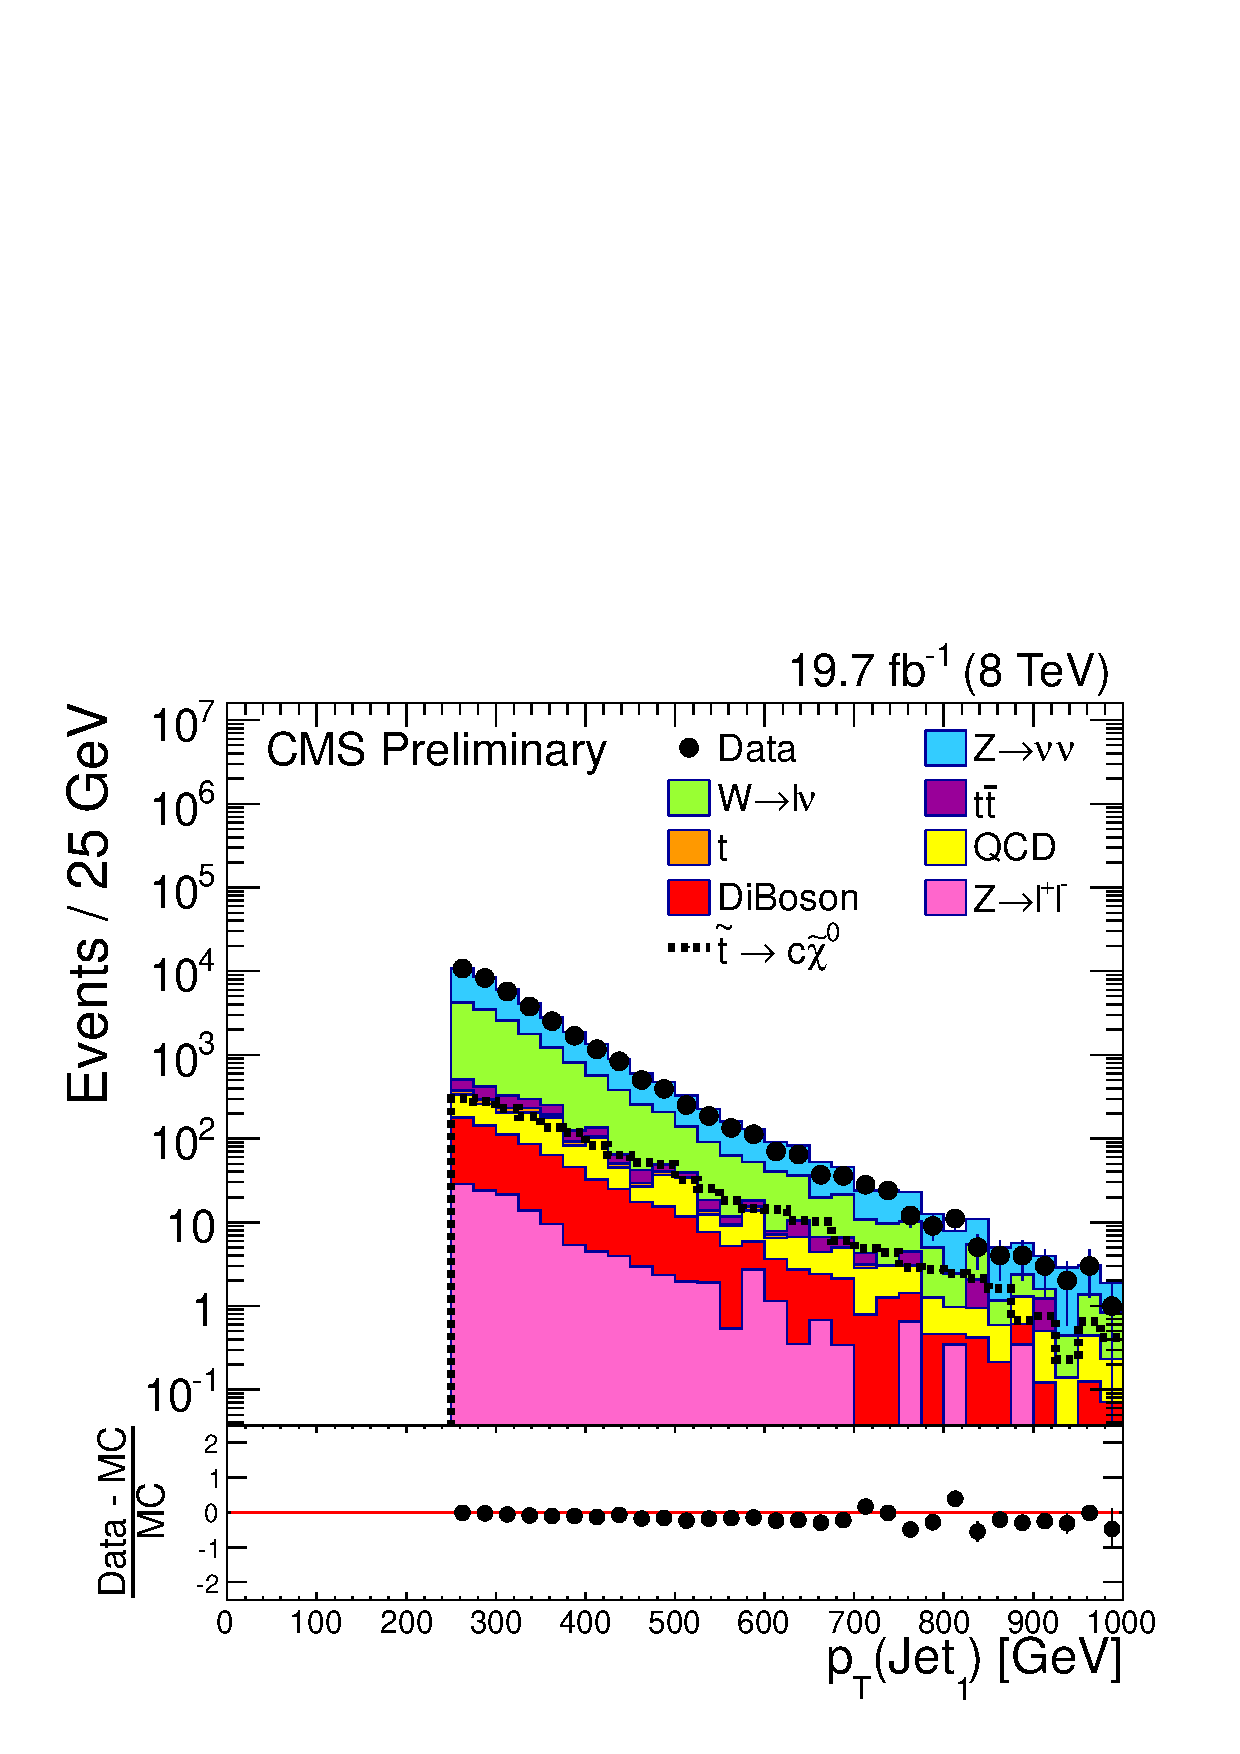
\includegraphics[scale=0.30]     {Figures/sus13009/cut/Jet1Pt.pdf}
  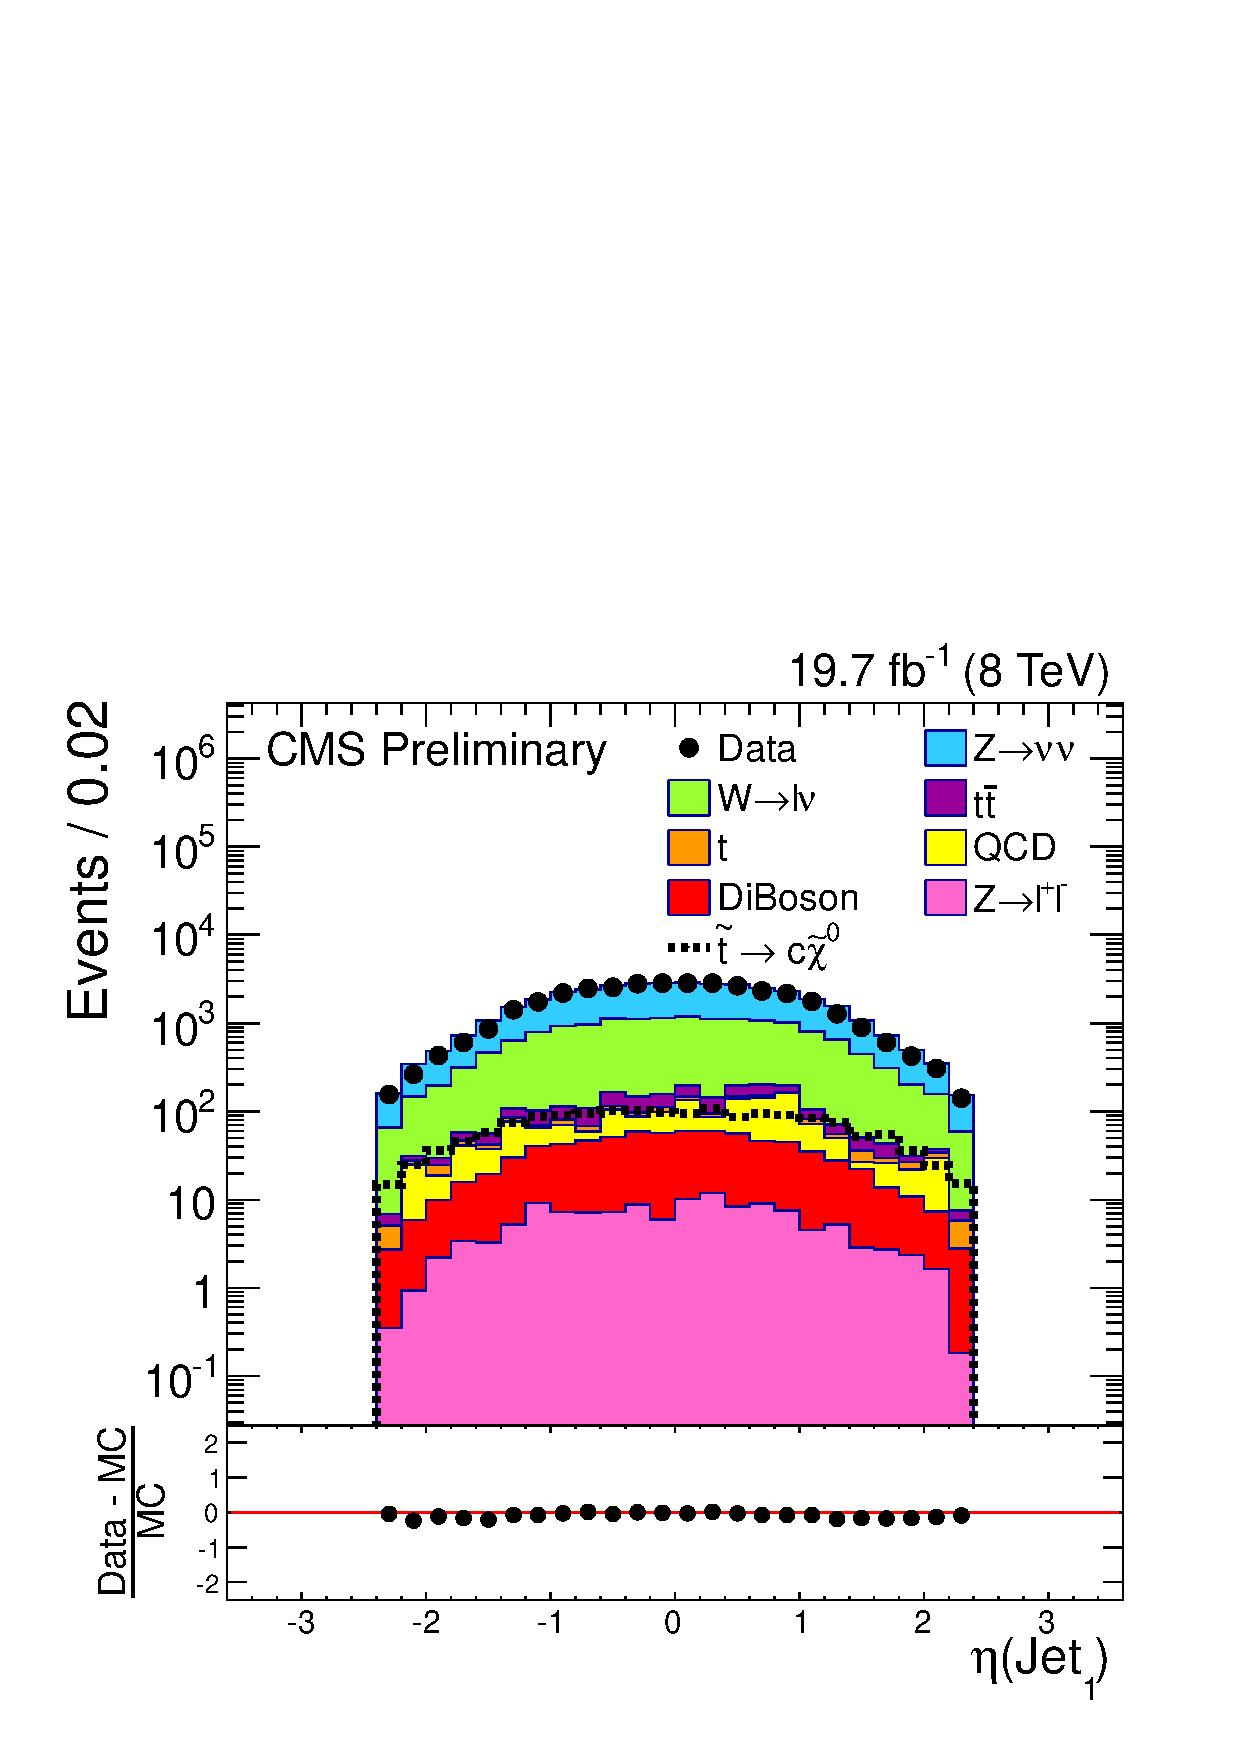
\includegraphics[scale=0.30]     {Figures/sus13009/cut/Jet1Eta.pdf}
  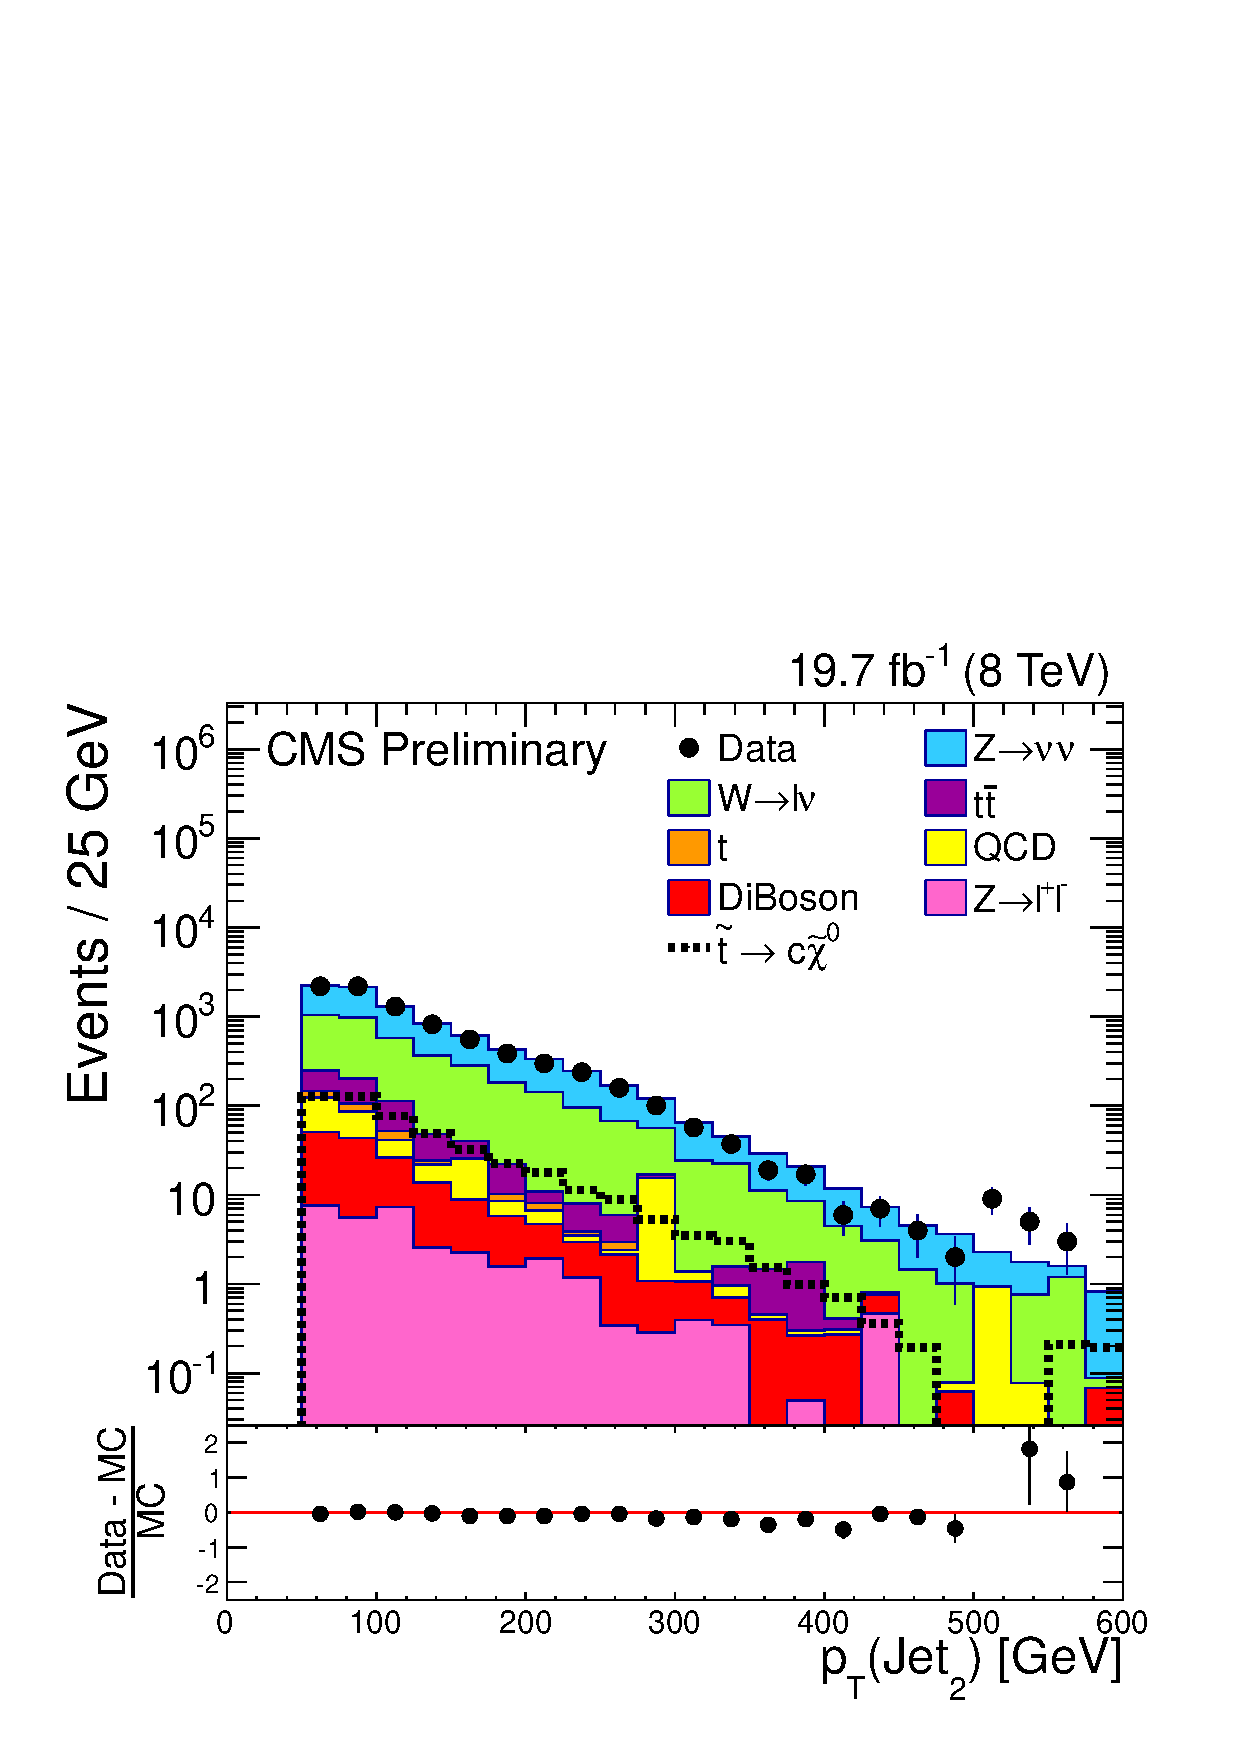
\includegraphics[scale=0.30]     {Figures/sus13009/cut/Jet2Pt.pdf}
  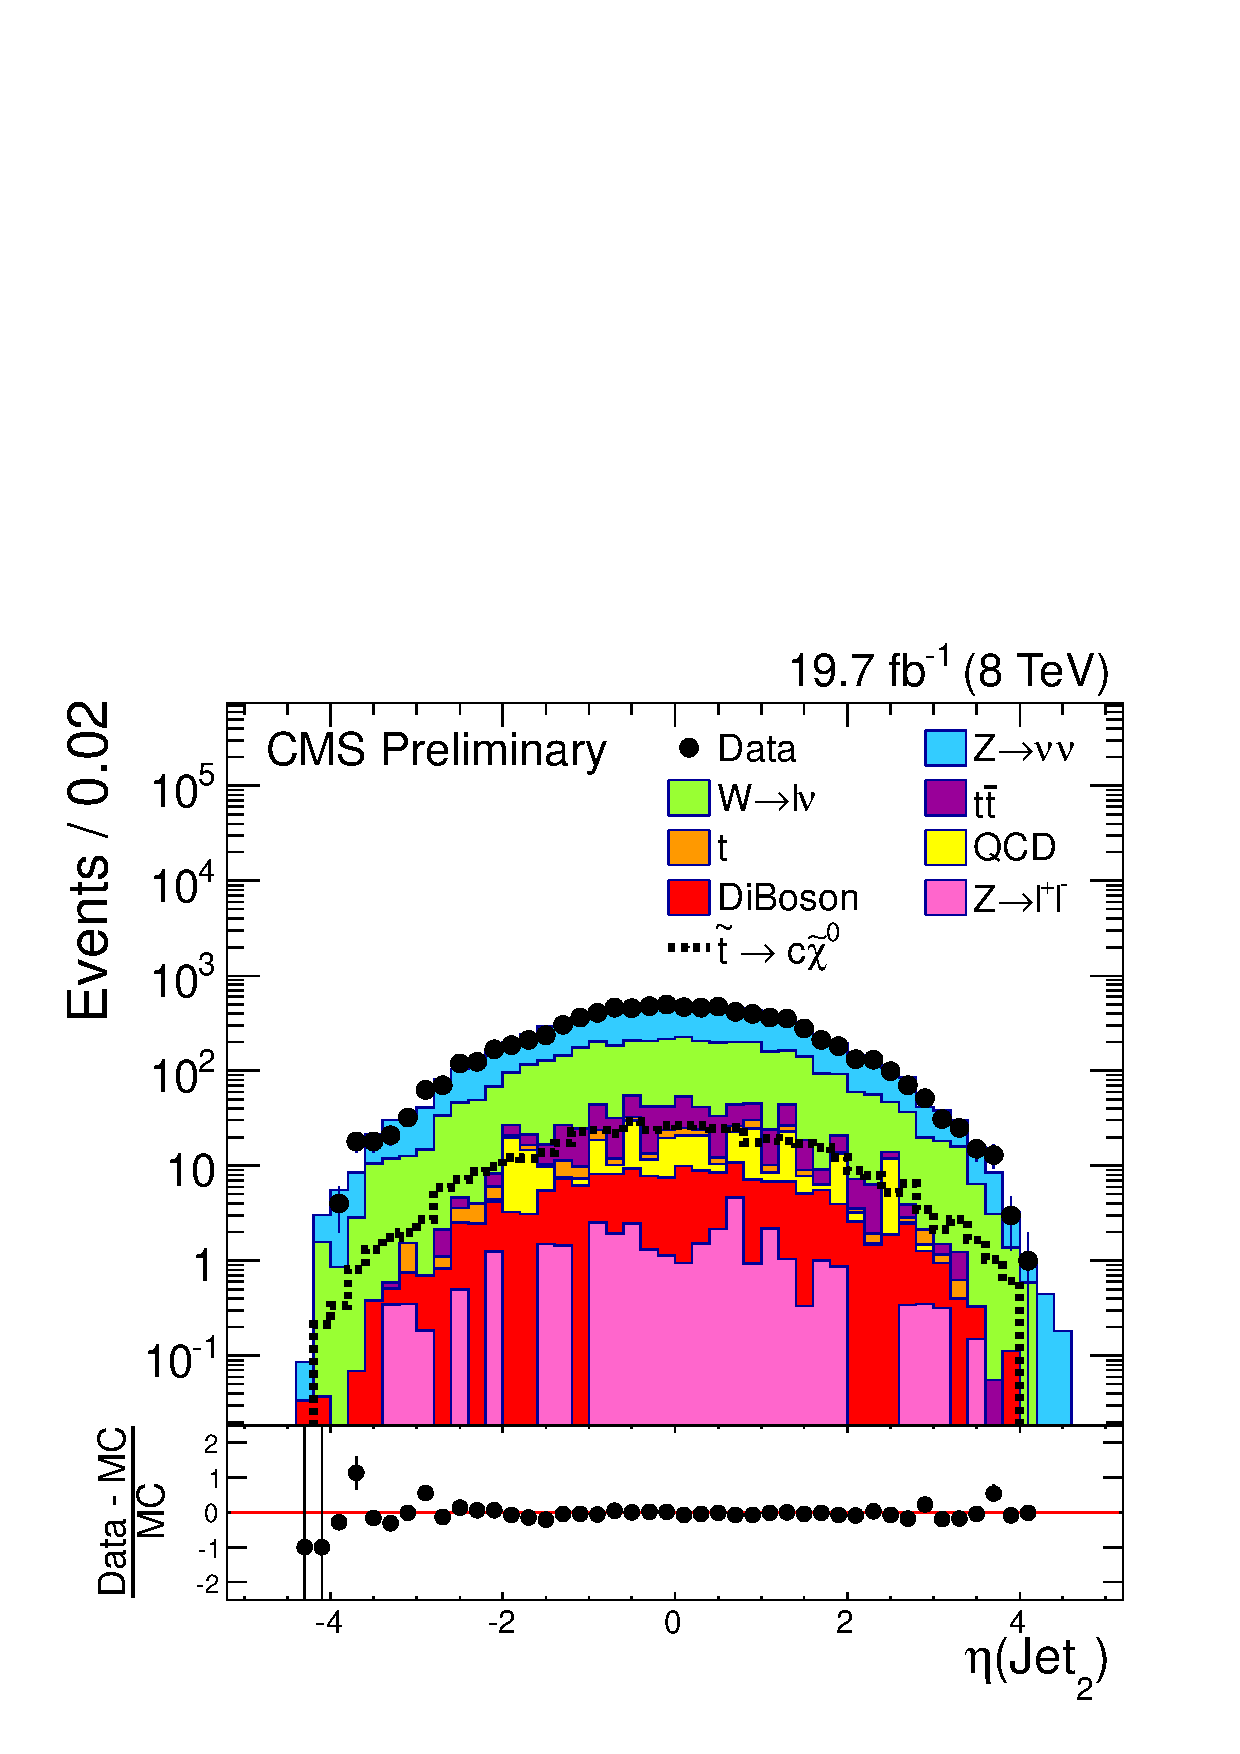
\includegraphics[scale=0.30]     {Figures/sus13009/cut/Jet2Eta.pdf}
   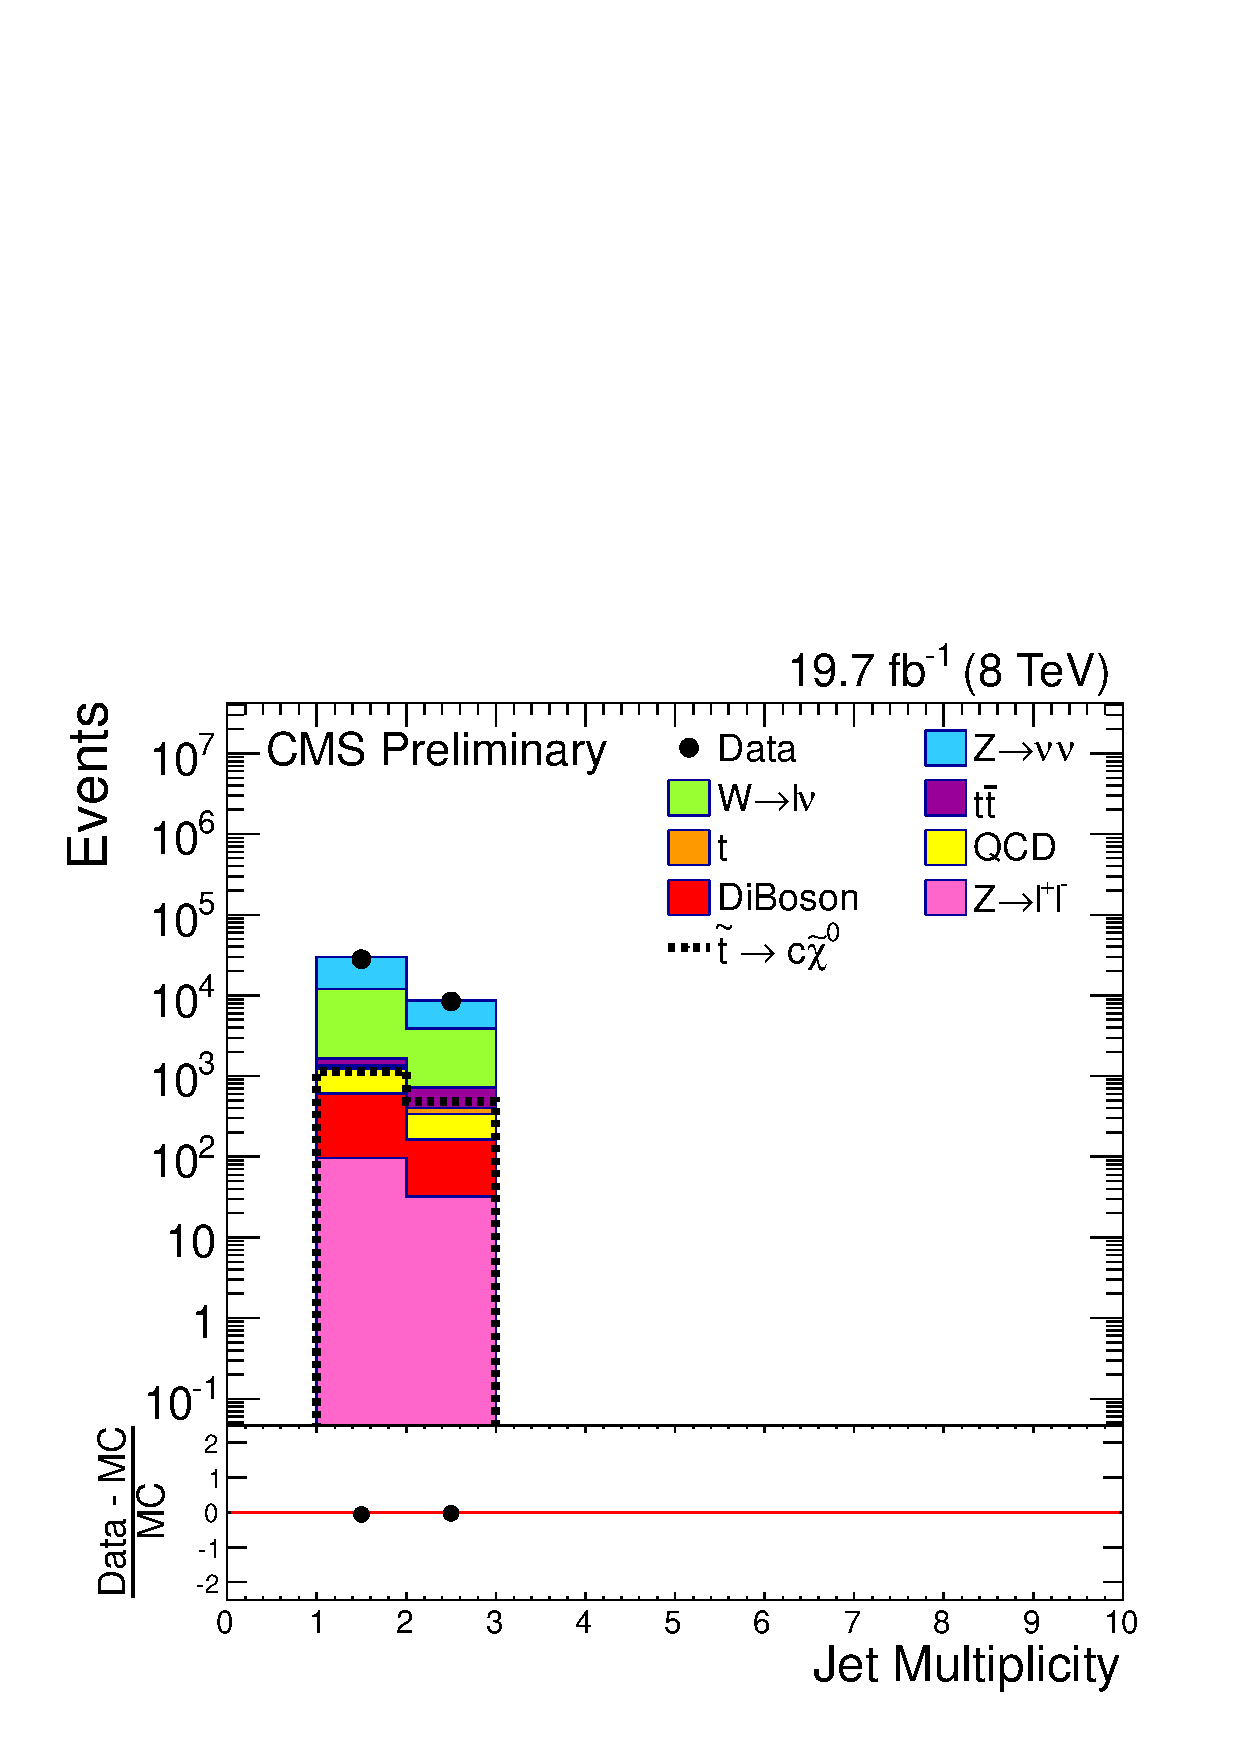
\includegraphics[scale=0.30]     {Figures/sus13009/cut/NJet.pdf}
   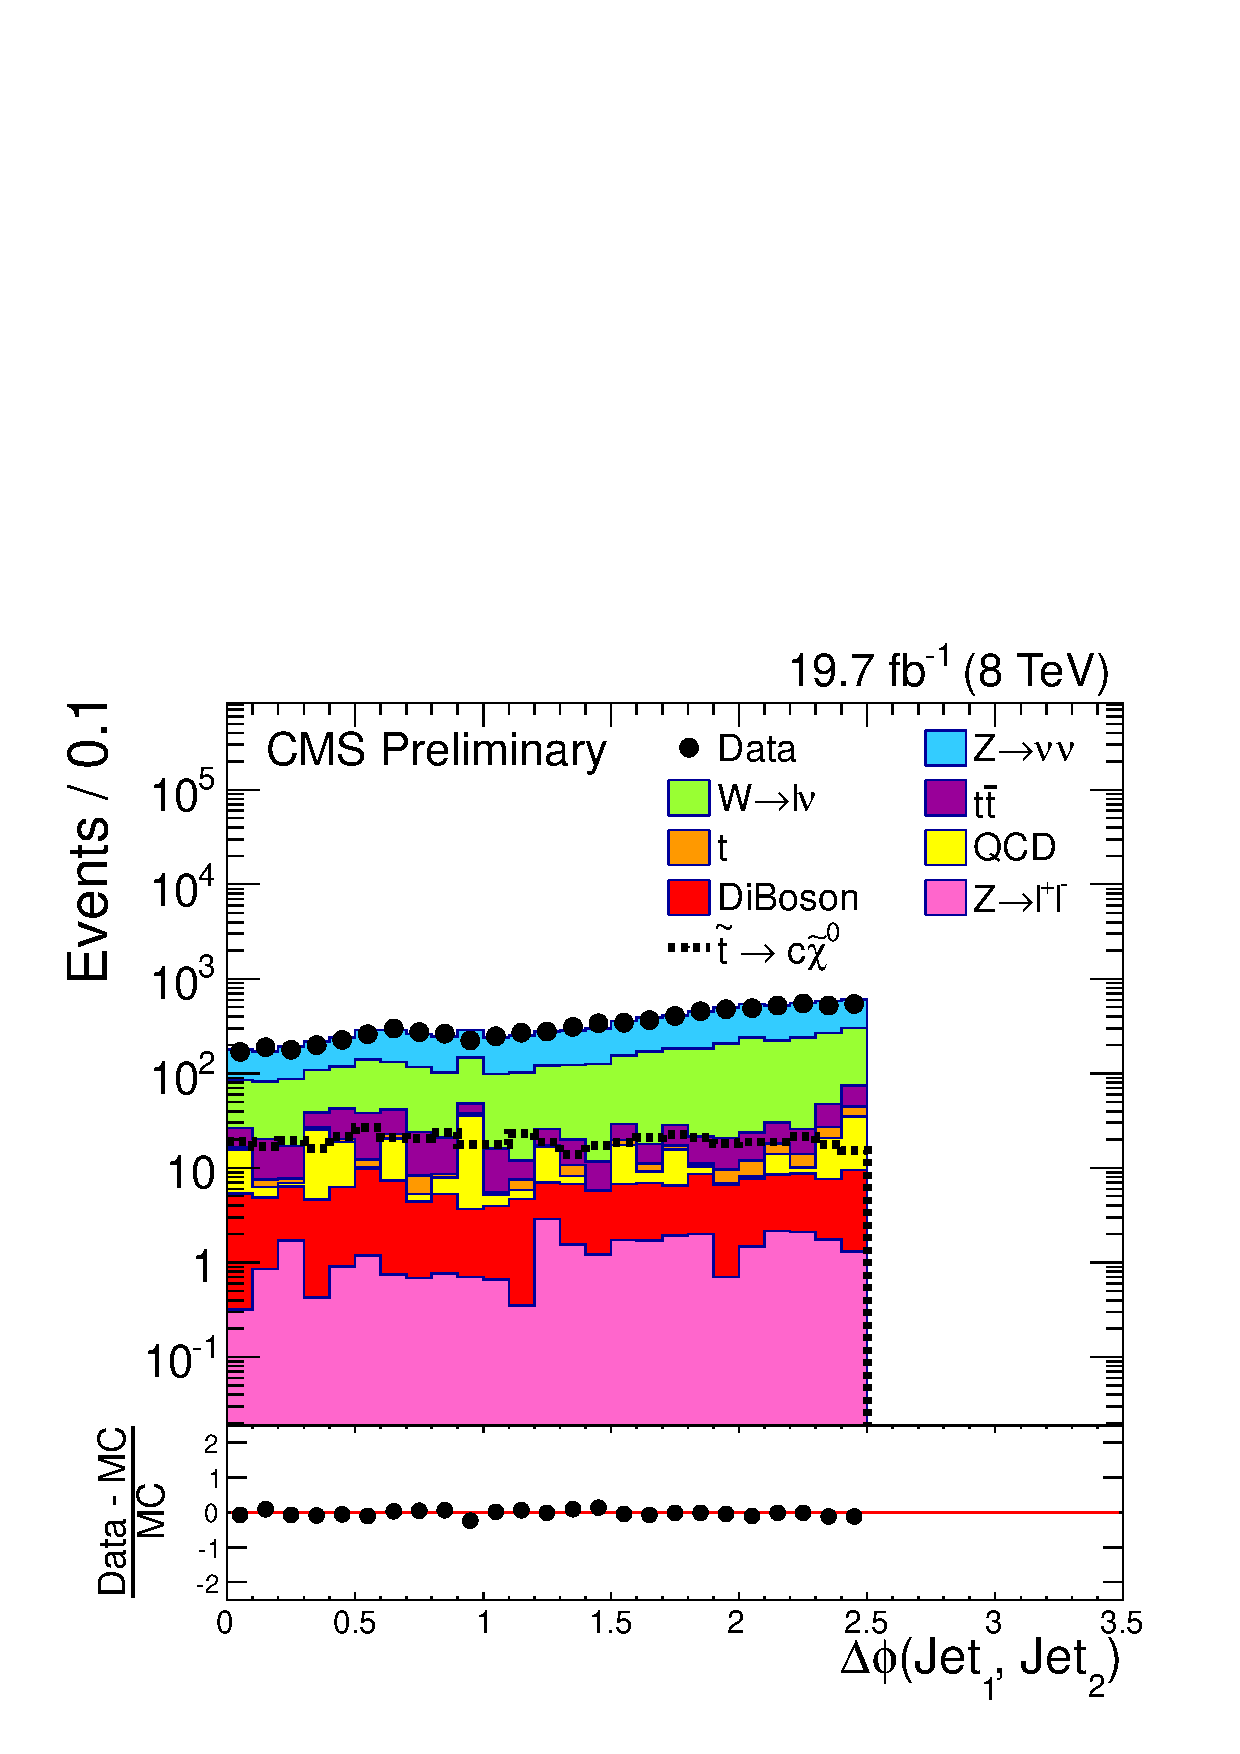
\includegraphics[scale=0.30]     {Figures/sus13009/cut/dPhi_Jet1_Jet2.pdf}
   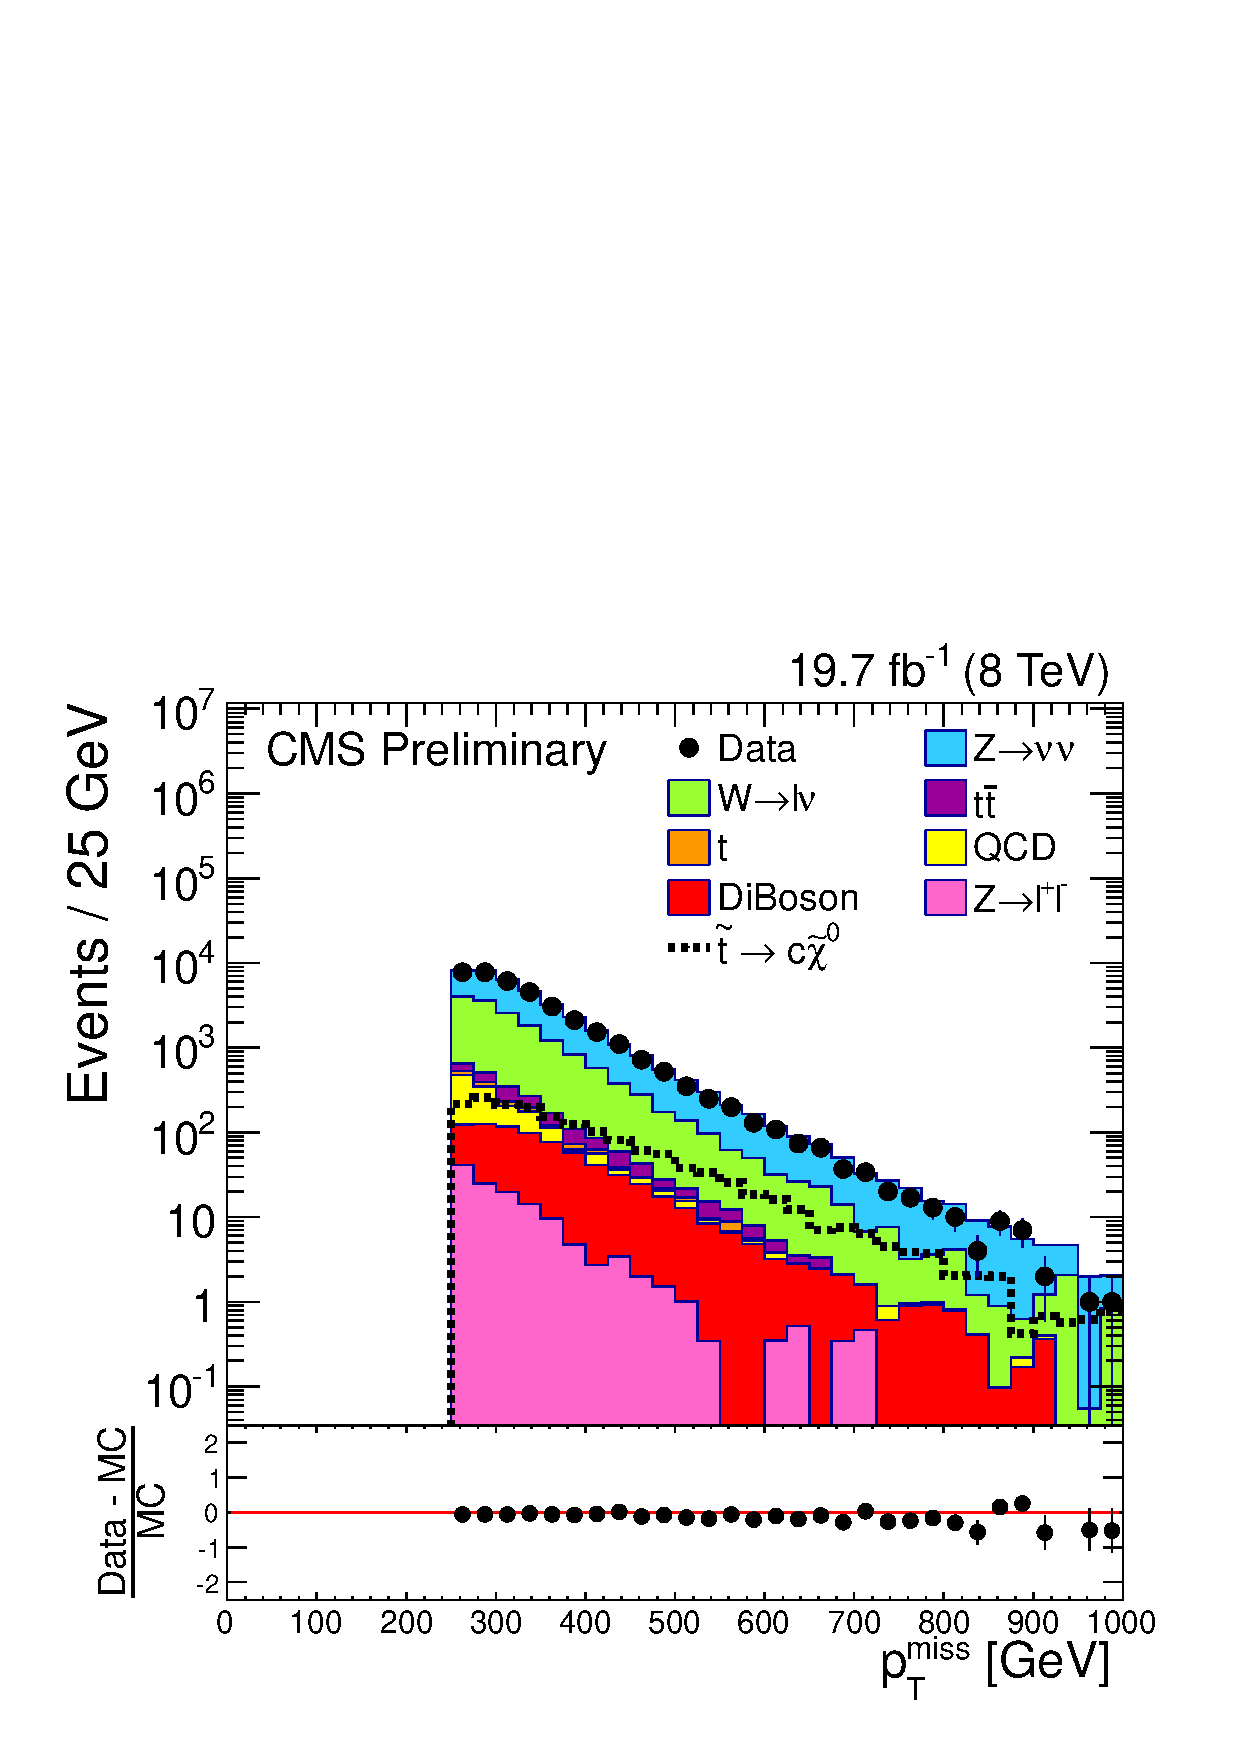
\includegraphics[scale=0.30]     {Figures/sus13009/cut/MetLep1.pdf}
   \caption{Plots of basic selection variables.  All figures except for the \pt and $\eta$ of the second leading jet are N-1 plots so all cuts are applied except the one being plotted (the leading jet $\pt$ cut for all plots except the jet $\pt$ and jet $\eta$ is set to 110 GeV). The leading SM backgrounds from \znunu\,+\,jets and \wpj events are normalised using a data-driven technique.%SM backgrounds are normalised as described in to data where available.
         \label{fig:ANA_Jet_selection_plots}}
  \end{center}
\end{figure}
%\begin{figure}[tb]
%  \begin{center}
%  \includegraphics[scale=0.35]     {cut/TIV.pdf}
%  \caption{Additional cleanup variables investigated.  We reject events with muons or electrons above 10\GeV and apply the TIV isolation as described in the text.
%         \label{fig:ANA_MuPt_and_TIV}}
%  \end{center}
%\end{figure}
A summary of all the selection criteria is given in Appendix~\ref{app:eventsel}.
Some of the kinematic distributions are shown in Figure~\ref{fig:ANA_Jet_selection_plots}.
%Fig.~\ref{fig:ANA_Jet_selection_plots} where the full monojet selection has been applied with a $\MET$ cut of 250 \GeV. All the distributions have been normalised as described in Appendix~\ref{app:normalisation}.

%The distribution of \MET for data and background after selecting monojet events and for a \MET cut of 250 \GeV is shown in Figure~\ref{fig:ANA_MET_plots}.

%We define the above described event selection with the \MET cut of 200 GeV as the baseline selection and subsequently apply tighter \MET\ selections of $\MET = 250, 300, 350, 400$ to obtain our search regions. 
%Optimisation studies have been performed for each of our signal samples to find the value of the \MET\ cut that gives the best expected limit. The study is documented in Appendix~\ref{app:opt_limit}. For both the ADD and dark matter signal points, the optimal \MET\ cut is found to be 350 \GeV. For Unparticles, the optimal \MET cut is found to be 300 \GeV or 350 \GeV, depending on the values of $d_U$. However the difference in expected limit is small and therefore a \MET\ cut of 350 \GeV is used for calculating limits, consistent with what is used for the ADD and dark matter signals.
%
%\begin{figure}[tb]
%  \begin{center}
%  \includegraphics[scale=0.45]{cut/Met.pdf}
%  \caption{The $\MET$ distribution after all selection cuts are applied for data and backgrounds.Representative signal distributions for dark matter, ADD and Unparticles are also overlaid. Events with $\MET > 1 \TeV$ are included in the overflow bin.}
%         \label{fig:ANA_MET_plots}  
%  \end{center}
%\end{figure}

Table \ref{tab:SEL_TabDataMC200} lists the number of events selected at each step of the analysis, for data and simulation.
\begin{table*}[htb] %table 7 v04 110811:05  
        \begin{center}
        \caption{Number of events selected at each step of the analysis, for data and simulation. Backgrounds are obtained from MC and normalised as described in Appendix~\ref{app:normalisation}.}%from $W$ and $Z$ use $\PYTHIA$8 with tune Z2 normalised to data, and with pile-up reweighting.} 
\label{tab:SEL_TabDataMC200}
 {\footnotesize
               \begin{tabular}{l|rrrrrrr|r} \hline
Selection     & \wpj & \zpj & \znunu\,+\,jets & Diboson &  $\ttbar$ &  Single top  &  QCD & Total BG   \\ \hline 
Cross section (pb) & 228.9  & 40.5   & 588.3  & 234.0  & 1.085e6  & 114.8  & 105.7  &   \\ \hline
%Generated events   & 1.27e7 & 2.66e6 & 1.45e7 & 6.86e6 & 4.27e7   & 7.06e6 & 2.98e7 &   \\ \hline
Trigger                        & 2514352 &  190332   & 4337526 &  65666  & 461413 & 77284 &  5429269 &  13075841 \\ 
$\MET >200$ \GeV               & 317656  &  30242    & 134578  &  9572   & 63174  & 9289  &  87605   &  652117   \\
Noise Cleaning                 & 292550  &  27880    & 123420  &  8706   & 59412  & 8525  &  81668   &  602162   \\
$\pt(\,\mathrm{j}_1)>$110~\GeV & 279323  &  26652    & 117513  &  8045   & 53353  & 7752  &  80844   &  573484   \\ 
$\njets \le 2$      	       & 254058  &  24413    & 109313  &  7287   & 29364  & 5596  &  44247   &  474278   \\ 
$\Delta\phi(j_1,j_2)<2.5$      & 237533  &  22947    & 104158  &  6984   & 25312  & 4815  &  8433    &  410181   \\ 
Muon veto                      & 106236  &  1511     & 104152  &  4051   & 9826   & 1892  &  7444    &  235112   \\ 
Electron veto                  & 79407   &  1004     & 104065  &  3459   & 6557   & 1325  &  7401    &  203218   \\ 
Tau veto                       & 71808   &  807      & 103106  &  3248   & 5599   & 1147  &  7047    &  192762   \\ \hline 
$\pt(\,\mathrm{j}_1)>$250 \GeV, 
& \multirow{2}{*}{13641}
& \multirow{2}{*}{127}   
& \multirow{2}{*}{22615}
& \multirow{2}{*}{639}
& \multirow{2}{*}{602}
& \multirow{2}{*}{172}
& \multirow{2}{*}{819}
& \multirow{2}{*}{38615}    \\
                $\MET>$250 \GeV   &        &           &          &         &         &        &           &           \\
$\pt(\,\mathrm{j}_1)>$300~\GeV   &6873    &  75       &11093     & 369     & 344     & 97     &  546      &  19397   \\ 
$\pt(\,\mathrm{j}_1)>$350~\GeV   &3182    &  40       &5231      & 206     & 178     & 49     &  332      &  9218    \\ 
$\pt(\,\mathrm{j}_1)>$400~\GeV   &1501    &  25       &2617      & 113     & 91      & 21     &  181      &  4549    \\ 
$\pt(\,\mathrm{j}_1)>$450~\GeV   &751     &  17       &1335      & 64      & 48      & 11     &  92       &  2318    \\ 
$\pt(\,\mathrm{j}_1)>$500~\GeV   &376     &  11       &727       & 36      & 27      & 5.2    &  61       &  1244    \\ 
$\pt(\,\mathrm{j}_1)>$550~\GeV   &204     &  7.4      &406       & 21      & 18      & 3.2    &  34       &  693     \\ \hline 
\end{tabular}} 
\end{center}
\end{table*}



\section{Data driven background estimation}
\label{sec:BKG}

The dominant backgrounds remaining after the monojet event selection are electroweak backgrounds from ``invisible $Z$'' decays and W\,+\,jets.
Both of these backgrounds are estimated from data by selecting a control sample of $\mu$+jet events, where \zmumu\,+\,jets is used to predict the invisible Z background and \wmunu\,+\,jets is used to predict the remaining W\,+\,jets background.
This muon control sample is derived from the same dataset as the signal.

The control samples are obtained by applying the full monojet selection with the exception of the lepton veto.
%Well-reconstructed 
%and isolated muons with $\pt(\mu)>20\GeV$  are selected following 
%the criteria described in Section~\ref{sec:ANA}.
To obtain a sample of \zmumu\ events, one well identified and isolated muon satisfying the selection in Section~\ref{sec:ANA} is required and the invariant mass of this muon with another reconstructed muon in the event is required to be between 60 and 120 GeV. 
%Compared to the previous version of the analysis, where the second muon was also required to be isolated and well identified, we  an increase of 20$\%$ in the statistics of the \zmumu\ sample.
A sample of \wmunu\,+\,jets is similarly obtained by requiring one well identified and isolated muon and with a reconstructed W transverse mass between 50 and 100 GeV.

Tables~\ref{tab:Zmuontable} and~\ref{tab:Wmuontable} show the event yields obtained for the \zmumu\ and \wmunu\ control samples and the predicted backgrounds from MC.

\begin{table*}[!Hhtb]  %table 8   110811:05  
        \begin{center}
\caption{Event yields for the \zmumu data control samples and the backgrounds from MC.
50\% uncertainty is assigned to each background (i.e. from \ttbar, single top, and diboson events) and these are combined in quadrature to get the total uncertainty on 
the number of background events in the \zmumu sample.}
\label{tab:Zmuontable}
{\small
                \begin{tabular}{l|ccccccc|cc} \hline
                          &\zpj & \wpj & \znunu\,+\,jets & \ttbar  & Single t & QCD    & Diboson &  All MC & Data\\\hline
%numbers on 1 Oct: new ntuple
$\pt(\,\mathrm{j}_1)>$250~\GeV  & 3067 & 0 &  0 & 37  & 5.7 & 0 & 68  & 3177 &  2547 \\
$\pt(\,\mathrm{j}_1)>$300~\GeV  & 1577 & 0 &  0 & 21  & 2.2 & 0 & 41  & 1641 &  1235 \\
$\pt(\,\mathrm{j}_1)>$350~\GeV  & 757  & 0 &  0 & 9.9 & 0.9 & 0 & 24  & 791  &   567 \\  
$\pt(\,\mathrm{j}_1)>$400~\GeV  & 382  & 0 &  0 & 4.8 & 0.9 & 0 & 13  & 401  &   277 \\
$\pt(\,\mathrm{j}_1)>$450~\GeV  & 198  & 0 &  0 & 0.7 & 0   & 0 & 8.2 & 207  &   150 \\
$\pt(\,\mathrm{j}_1)>$500~\GeV  & 109  & 0 &  0 & 0   & 0   & 0 & 4.4 & 113  &   79  \\ 
$\pt(\,\mathrm{j}_1)>$550~\GeV  & 62   & 0 &  0 & 0   & 0   & 0 & 2.6 & 65   &   40  \\ \hline
                 \end{tabular}}                                                                                   
\end{center}
\end{table*}



\begin{table*}[!Hhtb]
        \begin{center}
\caption{Event yields for the $W \rightarrow \mu \nu$ data control samples and the backgrounds from MC.
50\% uncertainty is assigned to each background (i.e. from $\Z$\,+\,jets, \ttbar, single top, QCD and diboson events) and these are combined in quadrature to get the total uncertainty 
on the number of background events in the $W \rightarrow \mu \nu$ sample.}
\label{tab:Wmuontable}
 {\small
  \begin{tabular}{l|ccccccc|cc} \hline
                         &\zpj & \wpj & \znunu\,+\,jets & \ttbar  & Single t & QCD  & Diboson  & All MC & Data\\\hline
%numbers 1July
$\pt(\,\mathrm{j}_1)>$250~\GeV  & 11436 & 183 & 0 & 608 & 158 & 0.3 & 197 & 12582  & 11371\\
$\pt(\,\mathrm{j}_1)>$300~\GeV  & 5712  & 94  & 0 & 313 & 80  & 0.3 & 121 & 6320   & 5477 \\
$\pt(\,\mathrm{j}_1)>$350~\GeV  & 2694  & 44  & 0 & 151 & 41  & 0.3 & 71  & 3001   & 2547 \\
$\pt(\,\mathrm{j}_1)>$400~\GeV  & 1349  & 22  & 0 & 76  & 22  & 0.3 & 41  & 1509   & 1258 \\
$\pt(\,\mathrm{j}_1)>$450~\GeV  & 712   & 9.9 & 0 & 41  & 13  & 0.3 & 22  & 798    & 668  \\
$\pt(\,\mathrm{j}_1)>$500~\GeV  & 389   & 6.6 & 0 & 20  & 7.8 & 0.3 & 13  & 437    & 352  \\
$\pt(\,\mathrm{j}_1)>$550~\GeV  & 223   & 3.7 & 0 & 11  & 4.8 & 0.3 & 6.5 & 249    & 184  \\ \hline 
                \end{tabular}}                                                              \end{center}
\end{table*}
A comparison between data and MC for the dimuon invariant mass and momentum after all the selection cuts and a \pt(j1) cut of 250 \GeV is shown in Figure~\ref{fig:BKGR_Z_mass}.%, where the missing transverse energy is redefined as the vector sum of the muon transverse momentum and missing transverse energy to emulate the missing energy in events where the lepton is lost.
\begin{figure}[!Hhtb]
  \begin{center}
  \includegraphics[scale=0.39]{Figures/sus13009/cut/ZleplepMT_60_120.pdf}
  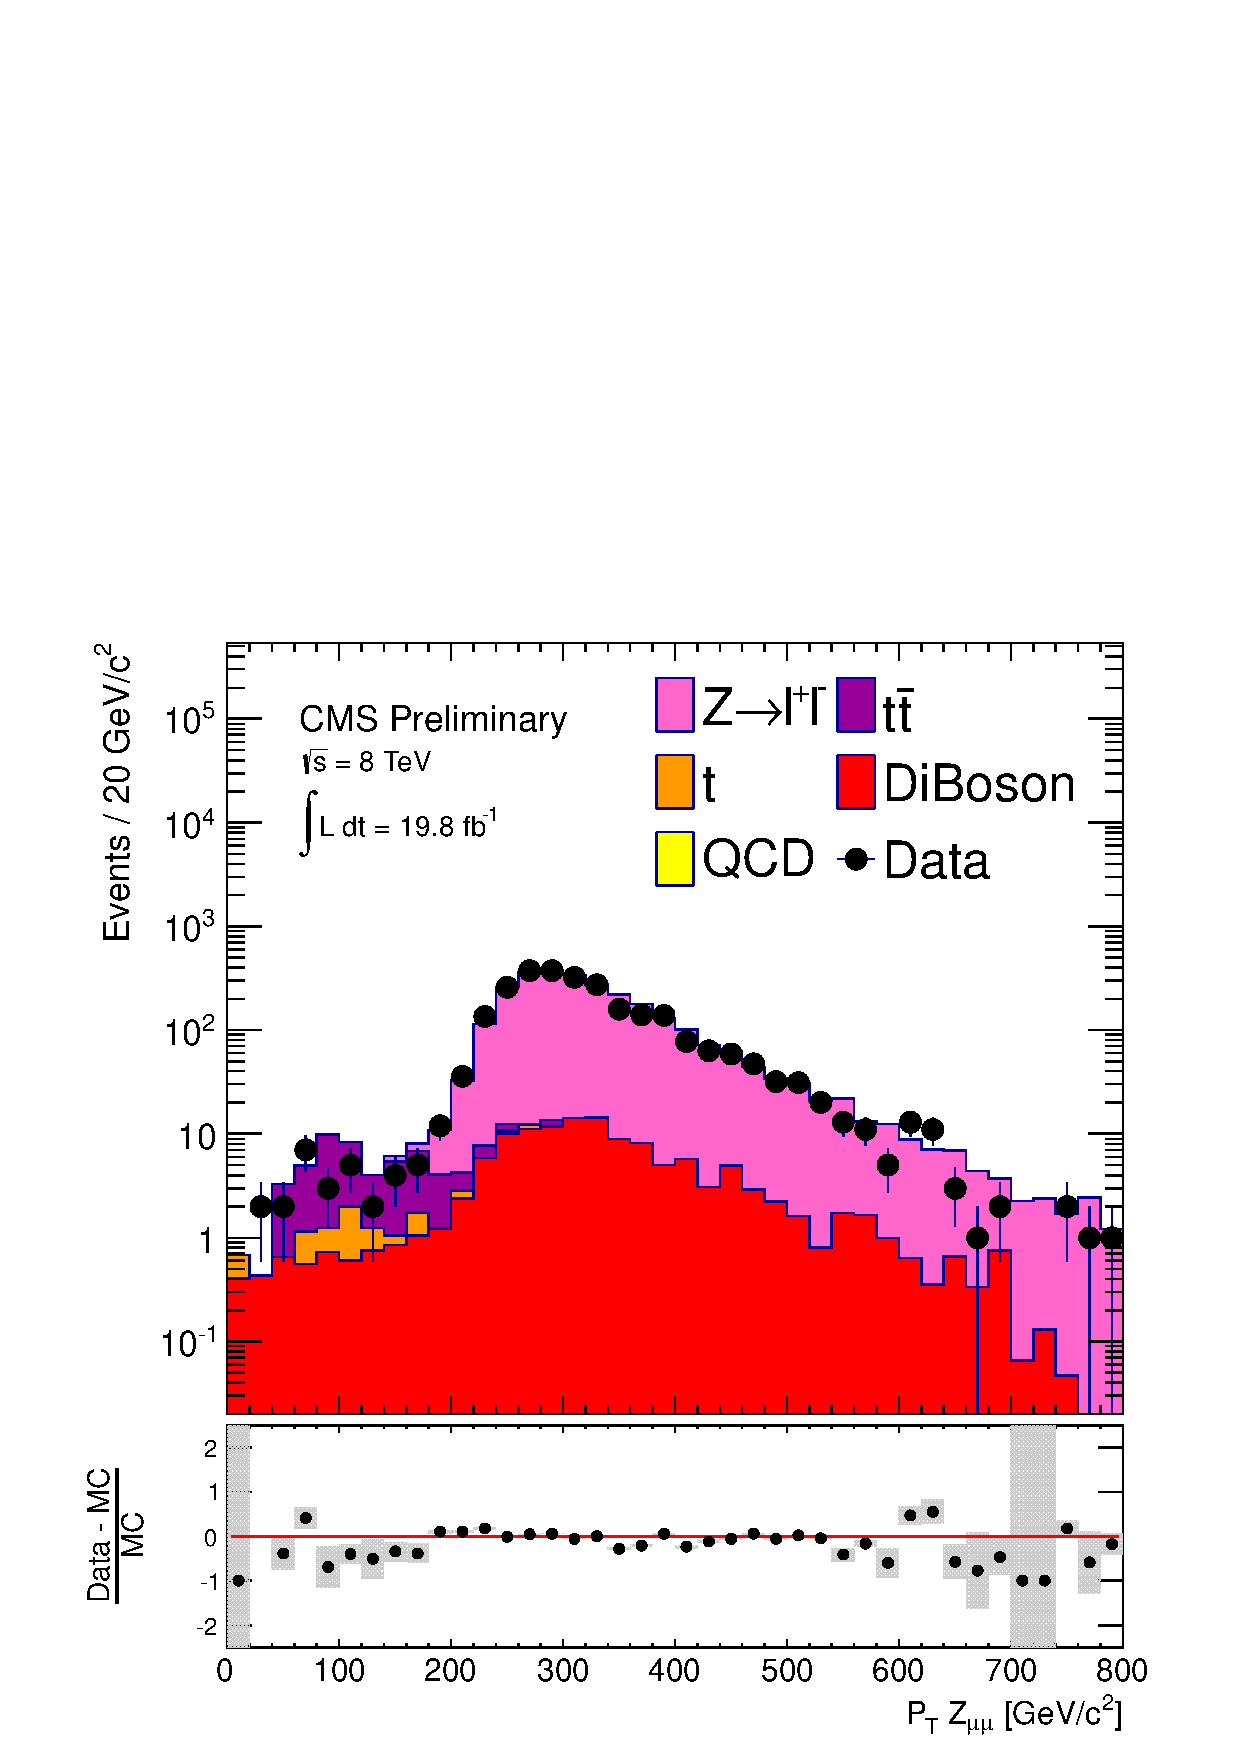
\includegraphics[scale=0.39]{Figures/sus13009/cut/ZleplepPT_60_120.pdf}
  \caption{Invariant mass and transverse momentum of the dimuon pair in the \zmumu control sample.}
  \label{fig:BKGR_Z_mass}
  \end{center}
\end{figure}

A comparison between data and MC for the transverse mass and momentum of the W after the full selection and for $\pt(\,\mathrm{j}_1) > 250 \GeV$ is shown in Figure~\ref{fig:BKGR_W_mass}.%, where the missing transverse energy is defined as the vector sum of the muon transverse momentum and missing transverse energy to emulate the missing energy in events where the lepton is lost.

\begin{figure}[!Hhtb]
  \begin{center}
  %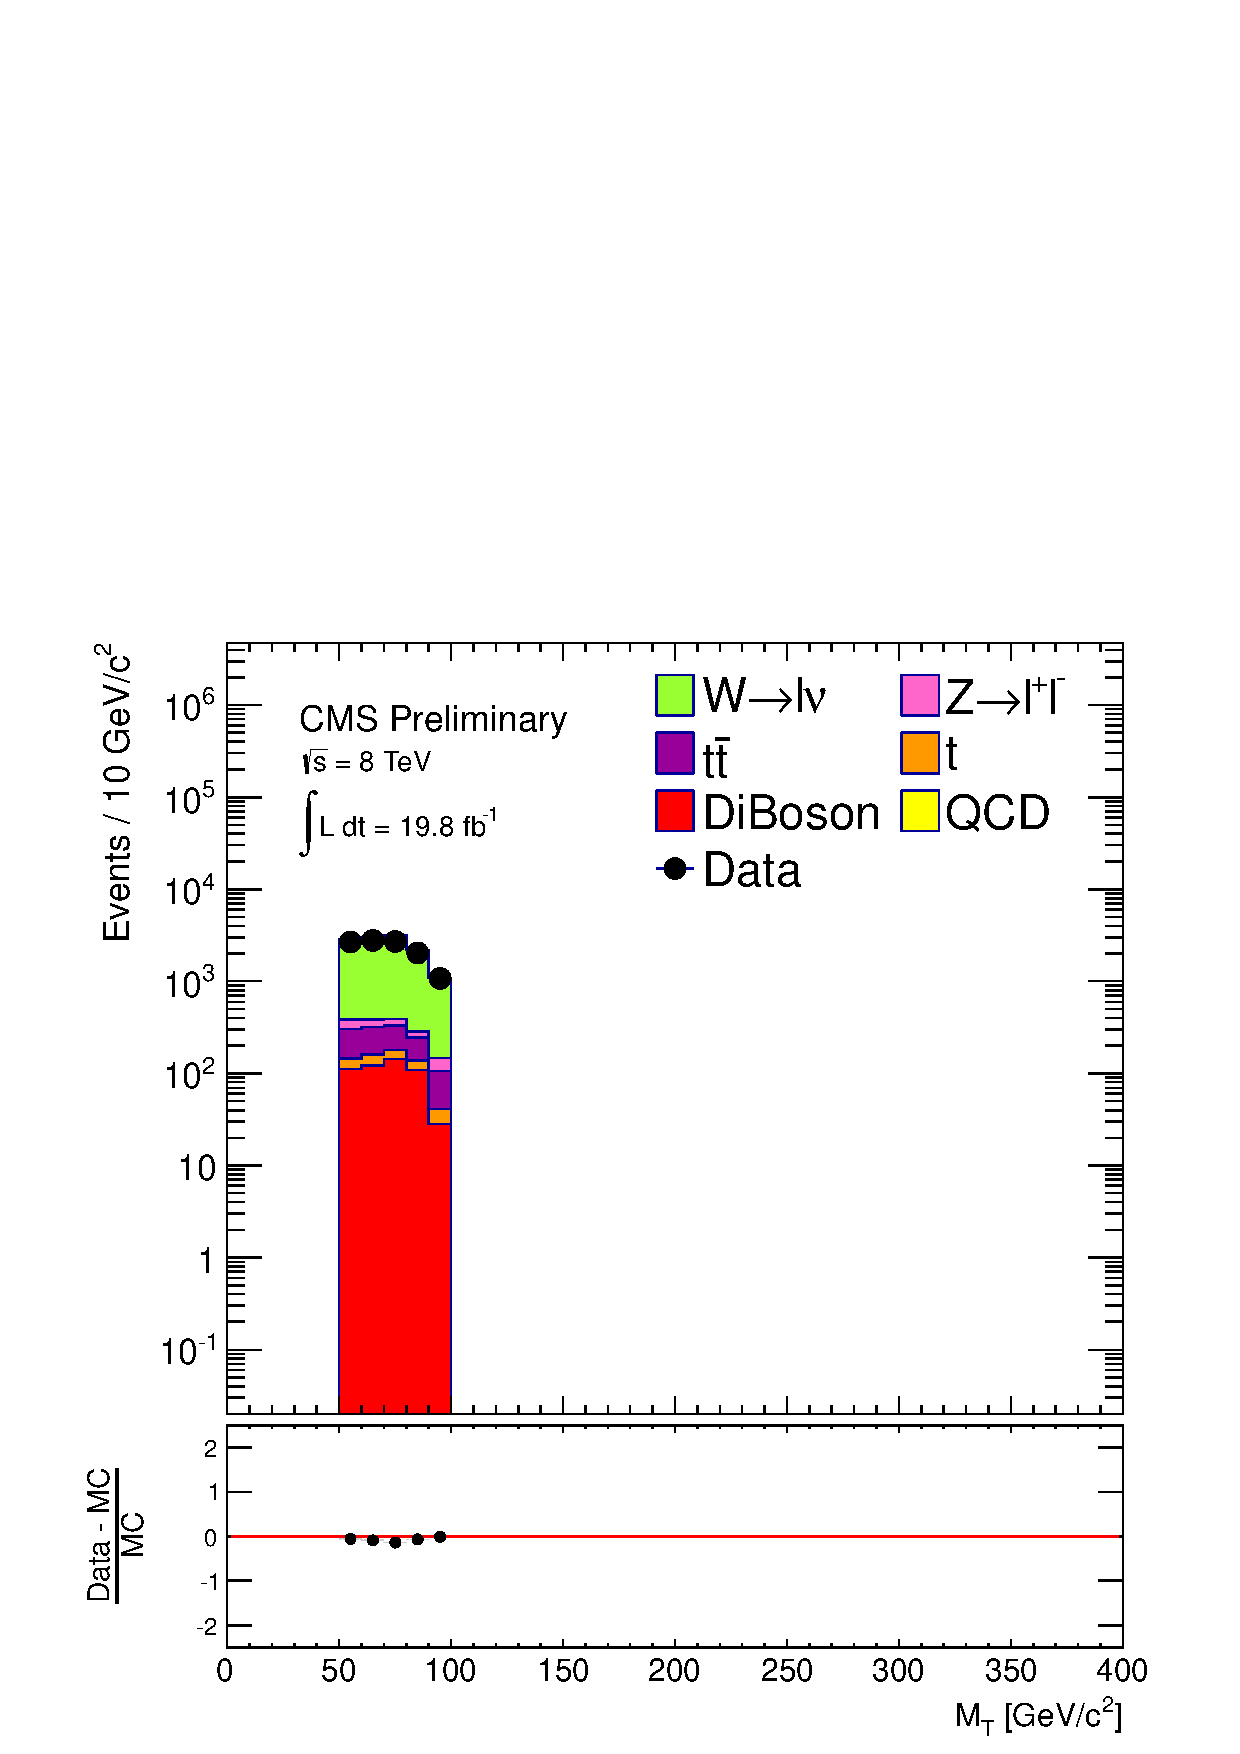
\includegraphics[scale=0.39]{cut/WlepnuMT_50_100.pdf}
  \includegraphics[scale=0.39]{Figures/sus13009/cut/WlepnuMT.pdf}
  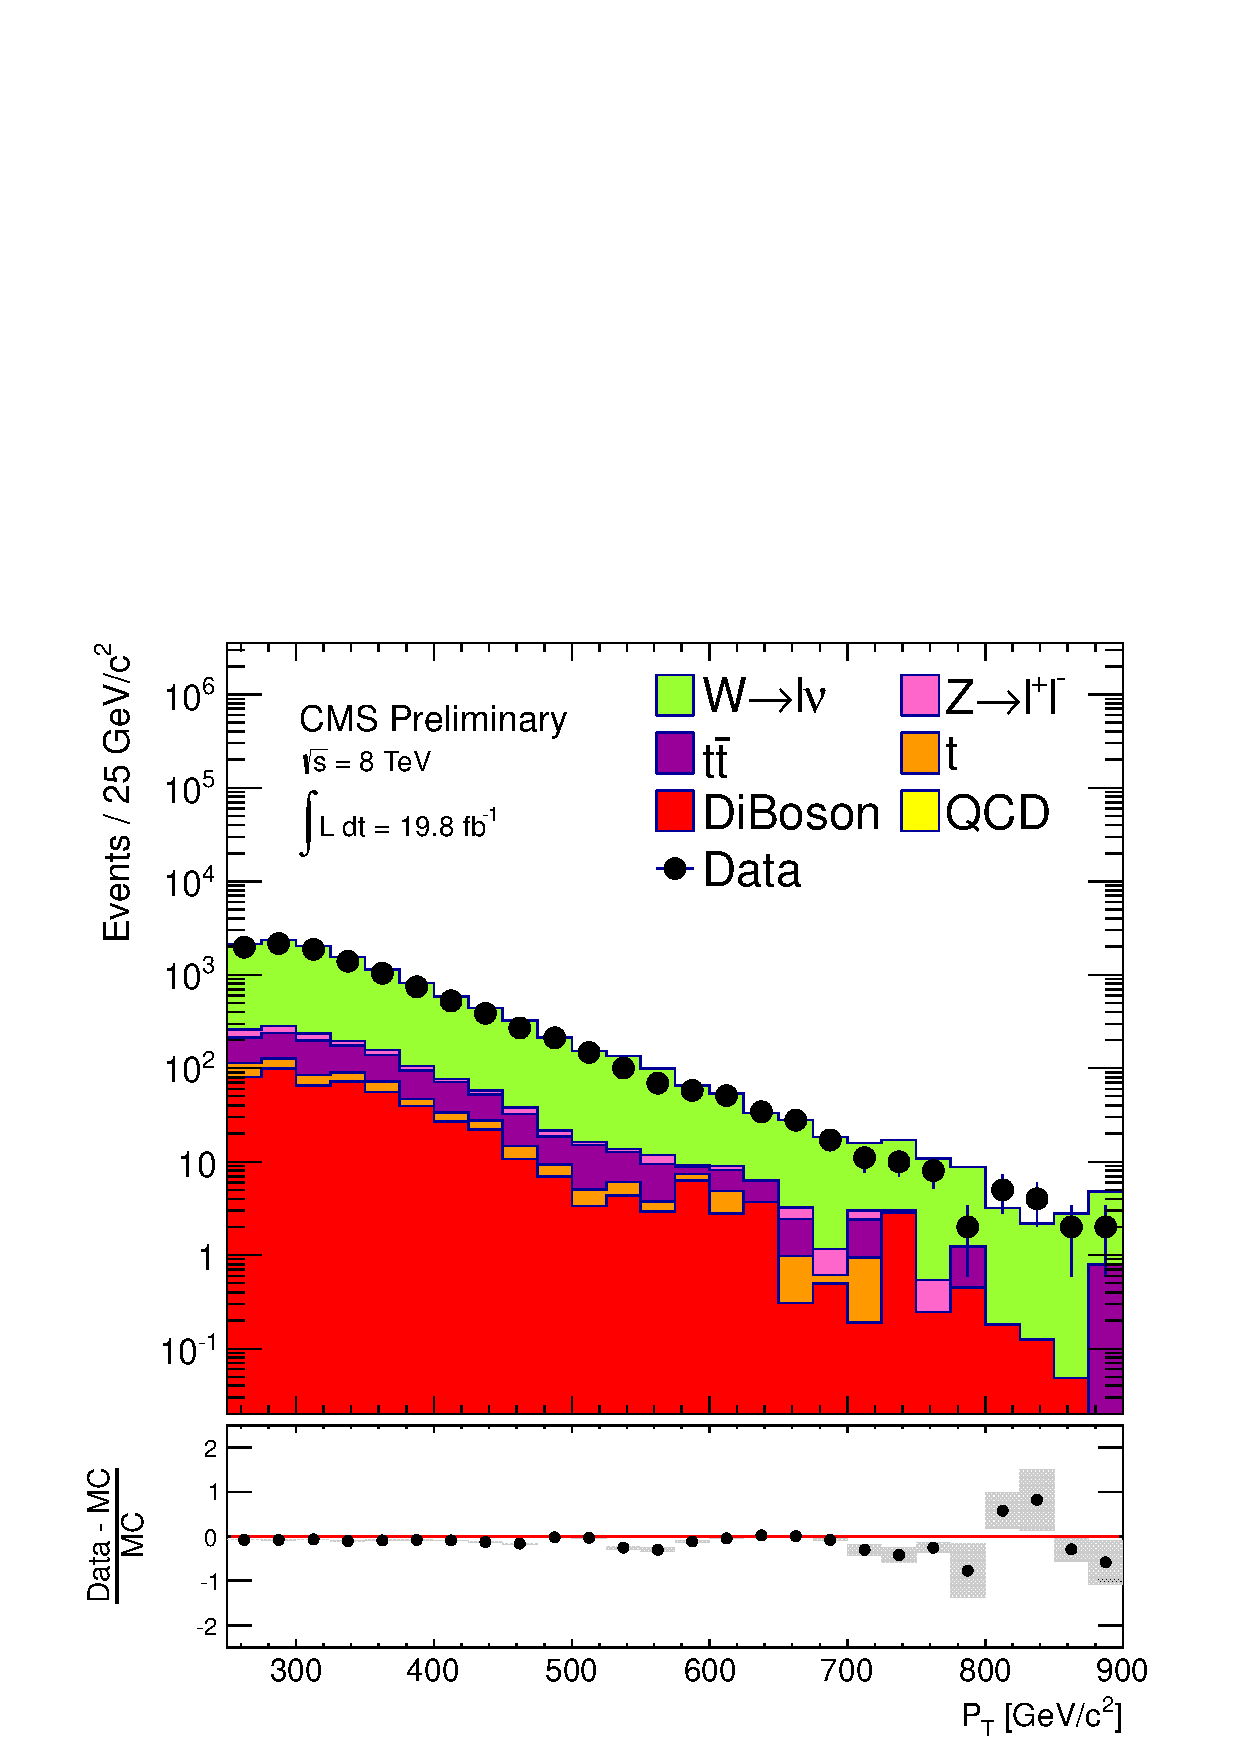
\includegraphics[scale=0.39]{Figures/sus13009/cut/WlepnuPT2_50_100.pdf}
  \caption{Transverse mass $M_{T}$ of the muon (left) and transverse momentum of $W^\pm$ candidates in the W mass window, $50 - 100 \GeV$ in the $W \rightarrow \mu \nu$ sample.}
  \label{fig:BKGR_W_mass}
  \end{center}
\end{figure}

\subsection{Estimation of \znunu background}

The \zmumu and \znunu events share similar kinematic characteristics and by interpreting the pair of muons as missing energy, the topology of the process in which the $Z$ boson decays to neutrinos can be reproduced.  The missing transverse energy in the \zmumu event is defined as the vector sum of the transverse momentum of the muons and the \MET. The number of \znunu events can then be predicted using:

\begin{equation}
N(Z\rightarrow\nu\nu) = \frac{N_{obs} - N_{bgd}}{A*\epsilon}\cdot R 
\end{equation}

where $N_{\rm obs}$ is the number of observed dimuon events, $N_{\rm bgd}$ is the number of background events contributing to the dimuon sample, $A$ is the fiducial and kinematic acceptance of the detector and the efficiency of the $Z$ mass window cut, $\epsilon$ is the selection efficiency of the event and $R$ is the ratio of branching fractions for the $Z$ decay to neutrinos and a pair of muons. These factors are determined as follows:
\begin{itemize}

\item $N_{bgd}$ : The dimuon sample comprises predominantly of \zmumu events with less than 1$\%$ contamination from background. The backgrounds are taken from Monte Carlo and a 50\% uncertainty is assigned to the number. 

\item $A$ : The acceptance $A$ is defined as the fraction of all generated events where the muons are reconstructed with $\pt > 20$ \GeV and $|\eta| < 2.1$ and the invariant mass of the muons is within 60 \GeV and 120 \GeV. This is obtained from Z\,+\,jets MC using generator level information.

\item $\epsilon$ : The event selection efficiency $\epsilon$ is defined as the efficiency of reconstructing muons passing all the identification and isolation criteria and with a reconstructed invariant mass between 60 and 120 $\GeV$, given that they are within the detector acceptance. 
The efficiency is taken from MC.
It is corrected by a scale factor to account for the difference in selection efficiency between data and MC.

\item $R$ : The ratio of the branching fraction $R = (\frac{BF(\znunubr)}{BF(\zmumubr)})$ is obtained from \cite{bib:BKG_PDG} and 
   is $5.942\pm 0.019$ when $l=\mu$. 
\end{itemize}
 
The selection of \zmumu events relies upon counting the number of events at each $\pt(\,\mathrm{j}_1)$ cut, which is correlated to the PF METnoMu.
We interpret the muons as missing energy, and add their $\pt$ into the PF MET in the redefinition of the \MET.
The momentum is balanced by $\pt(\,\mathrm{j}_1)$.
This exploits the similar kinematics of \znunu and \zmumu events, treating the muons as neutrinos. 
The estimate of METnoMu and $\pt(\,\mathrm{j}_1)$ therefore relies upon successfully identifying both muons in the muonic Z decay, 
in order to add them into the \MET and imitate an invisible Z decay where of course both neutrinos contribute to the \MET and so $\pt(\,\mathrm{j}_1)$. 

If either (or both) muons in a \zmumu decay is not properly identified, 
for example the muon does not pass identification requirements but the track is reconstructed, 
the energy of the muon will be included within the PF MET calculation and our procedure does not remove it. 
This event is likely to fail a METnoMu or $\pt(\,\mathrm{j}_1)$ cut.
It will not contribute to the total number of \zmumu events and therefore reduce the total \znunu estimation.
However, if it had of been a \znunu event, 
both neutrinos would lead to genuine missing energy and so in missing such events we have under-estimated the \znunu background.

In order to correct for this effect we count the number of events in MC where METnoMu /\pt gen Z $< 0.7$ in each inclusive $\pt(\,\mathrm{j}_1)$ bin. 
A threshold value of 0.7 is chosen as the Z resolution is $\sim 0.3$ and we wish to count events in the tail of the Z mass spectrum.
This gives an estimate of the number of events where we have not properly measured or identified one or two of the muons. 
The ratio, typically $<5\%$, is calculated in each $\pt(\,\mathrm{j}_1)$ bin and combined with the difference in efficiency for a TL or TT muon selection.
A correction factor dependent on the signal region of order 5\% is therefore applied.

%In addition, a 4.7$\%$ correction is applied to the predicted \znunu background to account for an inefficiency in \zmumu\ events where the muon track is reconstructed but the muon is not identified. These events were studied by plotting the ratio of \MET and the generated $Z$ boson \pt, they are present in the low tail of the distribution, below around 0.7, in \zmumu\ events but absent in the same distribution for \znunu events. 
%We therefore estimate the selection efficiency using Z\,+\,jets MC and assign a systematic of 2$\%$ to cover the variation of the data-MC scale factor from 1.0, measured in~\cite{bib:AN-11-240}.

A correction factor is also applied to R, to account for contamination from $g^{*}$. 
   $\alpha$ is the fraction of $g^{*}$ component in the Z, found from the difference in normalised \zmumu and \znunu samples in the Z mass window.
   $\beta$ is the fraction of events lying outside the Z mass window in \znunu MC.
   The $g^{*}$ contamination can be estimated using
   \begin{equation}
    g^{*} fraction = \frac{1-\alpha}{1-\beta} 
   \end{equation}
Normalised across all $\pt(\,\mathrm{j}_1)$ bins, we find a correction factor of 1.017.


Table~\ref{tab:Zinv_factors} shows the observed \zmumu event yields and the correction factors for various \MET\ cuts. Also shown is the estimated \znunu background and the total uncertainty on it. 
%A summary of the fractional contributions of the uncertainties to the total error on the \znunu background is shown in Table~\ref{tab:Z_jets_sys}. 
%The dominant contribution to the uncertainty is the statistical uncertainty from the size of the \zmumu sample. 

%For the baseline selection, this is found to be 14131.5$\pm$xxxxx. This can be compared to the prediction from the invisible Z MC, 14728.9$\pm$xxxx.

\begin{table*}%[!Hhtb]  %table 8   110811:05  
        \begin{center}
\caption{Summary of the \zmumu event yields and the efficiency factors used to predict the \znunu\,+\,jets background.}
\label{tab:Zinv_factors}
\small
       \begin{tabular}{l|ccccccc} \hline
%& & & & \MET\ cut&  & &  \\
$\pt(\,\mathrm{j}_1)$ (\GeV) & $>$ 250 & $>$ 300 & $>$ 350 & $>$ 400& $>$ 450  & $>$ 500 & $>$ 550 \\ \hline 
N$_{obs}$ & 2547 &  1235 &  567&  277 & 150 & 79  & 40  \\ 
N$_{bgd}$ & 111  &  64   &  35 &  19  & 8.9 & 4.4 & 2.7 \\ 
Acceptance $A$        & 0.805  & 0.833  & 0.851  & 0.864  & 0.881  & 0.905  & 0.896  \\
Efficiency $\epsilon$ & 0.862  & 0.843  & 0.822  & 0.802  & 0.775  & 0.751  & 0.754  \\
%R &         5.942 & 5.942 & 5.942 & 5.942 & 5.942 & 5.942 & 5.942  \\ 
g* corr. factor & 1.017 & 1.017 & 1.017 & 1.017 & 1.017 & 1.017 & 1.017\\ 
\hline
\znunu &21209$\pm$1115  &10077$\pm$592 &  4597$\pm$324 & 2250$\pm$197 & 1250$\pm$137 & 663$\pm$94 & 334$\pm$65 \\ \hline
       \end{tabular}                                                                                   
\end{center}
\end{table*}


\begin{table*}%[!Hhtb]  %table 8   110811:05  
        \begin{center}
\caption{Summary of the contributions to the total uncertainty on \znunu\,+\,jets background from the various factors used in the data-driven estimation.}
\label{tab:Z_jets_sys}
                \begin{tabular}{l|ccccccc} \hline
$\pt(\,\mathrm{j}_1)$ (\GeV) & $>$ 250 & $>$ 300 & $>$ 350 & $>$ 400& $>$ 450  & $>$ 500 & $>$ 550 \\ \hline 
Statistics (N$^{obs}$)  & 2.1 &  3.0 &  4.5 &  6.5 &  8.7 &  12  &  17 \\
Background (N$^{bgd}$)  & 1.6 &  2.0 &  2.4 &  2.7 &  2.9 &  2.9 &  3.5\\ 
Acceptance              & 2.0 &  2.1 &  2.1 &  2.2 &  2.4 &  2.5 &  2.9\\
Efficiency              & 2.1 &  2.1 &  2.3 &  2.6 &  3.3 &  4.4 &  5.5\\
R                       & 2.0 &  2.0 &  2.0 &  2.0 &  2.0 &  2.0 &  2.0\\ \hline
Total                   & 5.3 &  5.9 &  7.0 &  8.8 &  11  &  14  &  19 \\  \hline 
\end{tabular}
\end{center}
\end{table*}


\subsection{Estimation of W\,+\,jets background}
The second most dominant background arises from W+jet events that are not removed by the explicit lepton veto cut. These can come from hadronically decaying taus or events in which the lepton (electron or muon) is not identified, not isolated or not within the acceptance region. 
Such events in which the electron, muon or hadronic tau are effectively `lost' are estimated by using the $W \rightarrow \mu\nu +$jets control sample. The \wmunu events are first corrected for the acceptance ($A'$) and efficiency of reconstructing the events ($\epsilon'$) in the detector to obtain the total number of generated events ($N_{tot}^{\mu}$). 
\begin{equation}
N_{tot}^{\mu} = \frac{N_{obs} - N_{bgd}}{A'\epsilon'} \label{eqn:Ntot}
\end{equation}

This is subsequently weighted by the inefficiency factors (detailed below) to obtain the predicted number of events that would not be rejected by the lepton veto and thus remain in the monojet sample.

The total number of $W \rightarrow \mu\nu +$jets events that are out of the acceptance and not identified/isolated can be written as:
\begin{equation}
N_{lost \mu} = N_{tot}^{\mu}*(1 - A_{\mu}\epsilon_{\mu}).
\end{equation}
%\begin{eqnarray}
%N_{!A}^{\mu} &=& N_{tot}^{\mu}*(1 - A_{\mu})\\
%N_{!\epsilon}^{\mu} &=& N_{tot}^{\mu}*A_{\mu}*(1 - \epsilon_{\mu})\\
%\end{eqnarray}
where $A_{\mu}$ is the acceptance and $\epsilon_{\mu}$ is the efficiency of the muon selection used in the lepton veto definition.

Similarly, for an estimation of the `lost' electron background, we start with $N_{tot}^{\mu}$ and multiply by the ratio of the 
$W \rightarrow \mu\nu +$jets and $W \rightarrow e \nu +$jets events that are predicted at the generator level in MC ($f_e$) 
to obtain $N_{tot}$ for electrons. The lost electron background is given by:
\begin{eqnarray}
N_{tot}^{e}&=& N_{tot}^{\mu}*f_e,\,\,\, {\rm where }\,\, f_{e} = \frac{N_{gen}^{e}}{N_{gen}^{\mu}}\\
N_{lost e} &=& N_{tot}^{e}*(1 - A_{e}\epsilon_{e})\\
\end{eqnarray}
where $A_{e}$ is the acceptance and $\epsilon_{e}$ is the efficiency of the electron selection used in the lepton veto definition.
The electron acceptance is obtained using generator level MC and the selection efficiency is also obtained from MC with an assumed data/MC scale factor of 1.0.% with an assigned systematic that covers the variation in efficiency between data and MC.
%Table~\ref{tab:wjetslost} summarises the estimated lost muon and electron background.
%A detailed table showing the various factors that are used to estimate this background is shown in Table~\ref{tab:wjets-summary}.

%The same procedure as that outlined in the above equations is then followed to obtain the number of events where the electron is not reconstructed/isolated or out of the acceptance. The electron acceptance is obtained using generator level MC and the selection efficiency is also obtained from MC with an assigned systematic that covers the variation in efficiency between data and MC.
%~\cite{bib:AN-11-240}.
The component of the \wpj background from hadronic tau events is estimated in the same way. The ratio of the generated \wmunu and hadronic tau events ($f_{\tau}$) is taken from MC and used to obtain $N_{tot}$ for tau events. This is subsequently weighted by the inefficiency of the tau selection used in the veto to obtain the 'lost' hadronic tau background.
\begin{eqnarray}
N_{tot}^{\tau}&=& N_{tot}^{\mu}*f_{\tau},\,\,\, {\rm where }\,\, f_{\tau} = \frac{N_{gen}^{\tau}}{N_{gen}^{\mu}}\\
N_{lost \tau} &=& N_{tot}^{\tau}*(1 - A_{\tau}\epsilon_{\tau})\\
\end{eqnarray}
The tau ID efficiency is estimated from MC with a data/MC scale factor of 1.0 and assigned an uncertainty of 6$\%$ as recommended by the Tau POG. 
The electron and muon discriminants in the Tau ID selection can also result in the Tau veto rejecting electron and muon events. The probability of an electron or muon to fake a tau is estimated from the W\,+\,jets MC and found to be negligible (below 0.1$\%$).
% No correction is made to these fake rates to account for data/MC differences as recommended by the Tau POG.  The Tau POG recommends an uncertainty of 5$\%$ on the electron fake rate for electrons in the Barrel and 10$\%$ for those in the Endcap and a 30$\%$ uncertainty on the muon fake rate. Since the fake rates are very small for our analysis, we assign 10$\%$ to electrons in both the Barrel and Endcap and the recommended 30$\%$ for muons. 
% Table~\ref{tab:wjetstau-summary} shows the tau acceptance and efficiency that are used to obtain the remaining tau hadronic background. More details on the tau acceptance, efficiency and fake rates at different stages of the monojet selection are given in Table~\ref{tab:wjets-hadronictau}. 

All of the above components can be summarised in a Master Equation for estimating the 'Lost' W background:
\begin{equation}
N_{lost} = \frac{N_{obs} - N_{bgd}}{A'\epsilon'}*\Big[(1 - A_{\mu}\epsilon_{\mu}) + f_{e}*(1 - A_{e}\epsilon_{e}) + f_{\tau}(1 - A_{\tau}\epsilon_{\tau})\Big]
\end{equation}

The factors in this equation used to estimate the lost muon, electron and hadronic tau backgrounds are detailed in Table~\ref{tab:wjetslost}.  A summary of the estimated remaining W+jet events in the monojet sample is shown in Table~\ref{tab:wjetstotal}.  


%The remaining component of the W\,+\,jets background which is not accounted for by this method is that from hadronically decaying tau. This is taken from W\,+\,jets MC and corrected by the data/MC scale factor obtained from \wmunu\ events.
%Since the control sample for this background estimation is obtained by relaxing the track isolation veto, we estimate the TIV efficiency from MC for all the \MET\ regions and apply this efficiency to obtain the final W\,+\,jets prediction. 


\begin{table*}%[!Hhtb]  %table 8   110811:05  

        \begin{center}
\caption{Estimation of the remaining W\,+\,jets background from the lost electron, muon and hadronic tau contributions.}
\label{tab:wjetslost}
 \begin{tabular}{l|ccccccc} \hline
% & & & Met cut&  & & & \\
$\pt(\,\mathrm{j}_1)$ (\GeV) & $>$250 &$>$300 & $>$350 & $>$400& $>$450  & $>$500 & $>$550 \\ \hline 
N$_{obs}$  & 11371 &  5477 & 2547 & 1258 & 668 &  352 &  184 \\
N$_{bgd}$  & 1146  &  608  & 307  & 160  & 86  &  48  &  26  \\
A'$\epsilon'$   & 0.345 &  0.345 &  0.341 & 0.346 &  0.349 &  0.361 &  0.371 \\
N$_{tot}^{\mu}$ & 29666 &  14125 &  6573  & 3176  &  1666  &  841   &  425   \\ \hline
  
Lost Muon & & & & & & & \\
A$_{\mu}\epsilon_{\mu}$ & 0.887 &   0.895 &   0.901 &   0.908 &   0.908&    0.906 &   0.907  \\
N$_{lost \mu}$          & 3350  &   1484  &   649   &   292   &   152  &    79    &   40     \\ \hline

Lost Electron & & & & & & & \\
A$_{e}$$\epsilon_{e}$ &0.615 &  0.684 &  0.734 &  0.771 &  0.793 &  0.815 &  0.823\\
f$_{e}$               &0.374 &  0.465 &  0.548 &  0.610 &  0.653 &  0.706 &  0.727\\
N$_{lost e}$          &4273  &  2077  &  958   &  444   &  225   &  110   &  55   \\ \hline

Lost Tau & & & & & & & \\
A$_{\tau}$$\epsilon_{\tau}$ & 0.253  & 0.284  & 0.298  & 0.296  & 0.294  & 0.341  & 0.325 \\
f$_\tau$                    & 0.212  & 0.235  & 0.235  & 0.228  & 0.212  & 0.201  & 0.195 \\
N$_{lost \tau}$             & 4704   & 2377   & 1083   & 510    & 249    & 112    & 56    \\ \hline


N$_{lost}$ & 12328$\pm$707 &  5939$\pm$366 & 2690$\pm$180 & 1246$\pm$92 &  627$\pm$52 & 301$\pm$29 & 150$\pm$18 \\ \hline

       \end{tabular}                                                                                   
\end{center}
\end{table*}

\begin{table*}[!Hhtb]  %table 8   110811:05  

        \begin{center}
\caption{Summary of the estimated total remaining W\,+\,jets background.}% and its comparison with the MC prediction.}
\label{tab:wjetstotal}
\small
 \begin{tabular}{l|rrrrrrr} \hline
% & & & Met cut&  & & & \\
$\pt(\,\mathrm{j}_1)$ (\GeV)  & $>$250 &$>$300 & $>$350 & $>$400& $>$450  & $>$500 & $>$550 \\ \hline 
N$_{tot}^{\mu}$     & 29666  &  14125  &  6573  & 3176   &  1666  &  841   &  425   \\ 
N$_{lost \mu}$      &  3350  &   1484  &   649  &  292   &   152  &   79   &   40   \\ 
N$_{lost e}$        &  4273  &   2077  &   958  &  444   &   225  &  110   &   55   \\ 
N$_{lost \tau}$     &  4704  &   2377  &  1083  &  510   &   249  &  112   &   56   \\ 
N$_{lost}$          & 12328$\pm$707 &  5939$\pm$366 & 2690$\pm$180 & 1246$\pm$92 &  627$\pm$52 & 301$\pm$29 & 150$\pm$18 \\ \hline
\end{tabular}
\end{center}
\end{table*}


The uncertainty on the W\,+\,jets estimation includes; the statistical uncertainty on the number of single-muon events in the data, a 50$\%$ uncertainty on the background events obtained from MC, an uncertainty on acceptance from PDFs (2\%) and MC statistics and an uncertainty on the selection efficiency $\epsilon$ from the variation in the data/MC scale factor and MC statistics. A summary of the fractional contributions of these uncertainties to the total error on the W\,+\,jets background is shown in Table~\ref{tab:wjetssys}. 
It is dominated by statistical uncertainty on $N_{obs}$ and 50\% uncertainties assigned to $N_{bkg}$.

\begin{table*}
        \begin{center}
\caption{Summary of the contributions (in \%) to the total uncertainty on the W\,+\,jets background from the various factors used in the data-driven estimation.}
\label{tab:wjetssys}
                \begin{tabular}{l|ccccccc} \hline
$\pt(\,\mathrm{j}_1)$ (\GeV)  & $>$250 &$>$300 & $>$350 & $>$400& $>$450  & $>$500 & $>$550 \\ \hline 
Statistics (N$_{obs}$) & 1.0 & 1.5 & 2.3 & 3.2 & 4.4 & 6.2 & 8.6  \\  
Background (N$_{bgd}$) & 3.3 & 3.7 & 4.0 & 4.2 & 4.2 & 4.3 & 4.4  \\ 
$A'$                   & 2.0 & 2.0 & 2.0 & 2.0 & 2.0 & 2.1 & 2.1  \\ 
$\epsilon'$            & 2.0 & 2.1 & 2.2 & 2.4 & 2.7 & 3.1 & 3.7  \\ 
$A_{\mu}$              & 0.1 & 0.1 & 0.2 & 0.2 & 0.3 & 0.4 & 0.5  \\ 
$\epsilon_{\mu}$       & 0.1 & 0.1 & 0.2 & 0.2 & 0.3 & 0.4 & 0.6  \\ 
$A_{e}$                & 0.7 & 0.9 & 1.0 & 1.1 & 1.2 & 1.3 & 1.3  \\ 
$\epsilon_{e}$         & 0.7 & 0.9 & 1.0 & 1.1 & 1.2 & 1.3 & 1.4  \\ 
$A_{\tau}$             & 0.2 & 0.2 & 0.2 & 0.2 & 0.2 & 0.3 & 0.3  \\ 
$\epsilon_{\tau}$      & 0.2 & 0.2 & 0.2 & 0.2 & 0.2 & 0.3 & 0.3  \\  \hline
Total                  & 5.7 & 6.2 & 6.7 & 7.4 & 8.2 & 9.7 & 12   \\  \hline 
\end{tabular}                                                                             
\end{center}
\end{table*}

%A summary of the fractional contributions of these uncertainties to the total error on the W\,+\,jets background is shown in Table~\ref{tab:W_jets_sys}.

%\begin{table*}%[!Hhtb]  %table 8   110811:05  
%        \begin{center}
%\caption{Summary of the contributions to the total uncertainty on W\,+\,jets background from the various factors used in the data-driven estimation.}
%\label{tab:W_jets_sys}
%                \begin{tabular}{l|ccccccc} \hline
% & & & & \MET cut & & & \\
%Source of Uncertainty  & 250 &300 & 350 & 400& 450  & 500 & 550 \\ \hline 
%Source of Uncertainty                          & $\MET > 250$ &$\MET > 300$ &$\MET > 350$ &$\MET > 400$ &   $\MET > 450$ & $\MET > 500$ & $\MET > 550$ \\ \hline 
%Statistics (N$_{obs}$) & 0.9 & 1.4 & 2.0 & 4.1 & 5.7 & 7.8 \\
%Background (N$_{bgd}$) & 7.8 & 6.8 & 5.7 & 5.8 & 5.8 & 5.4 & 7.3 \\
%Acceptance (A') & 2.0& 2.0 & 2.0 & 2.1 & 2.1 & 2.2 &  2.3 \\
%Selection efficiency ($\epsilon'$) & 2.1 & 2.2 & 2.5 & 2.9 & 3.6 & 4.6 & 5.9 \\
%Total & 
%        \end{tabular}                                                                                   
%\end{center}
%\end{table*}

\subsection{QCD Background Estimation}
\label{section:QCD}
The QCD background is predicted using MC, with a scale factor derived from a QCD rich control region.
The standard monojet event selection is applied to events, apart from those cuts which remove the majority of the QCD: $\Delta \phi(\,\mathrm{j}_1, \,\mathrm{j}_2)<2.5$ and $N_{jets} < 3$.
The $\pt$ requirement used to count jets is varied between 20 and 80 \GeV. 

\begin{figure}[htbp!]
\begin{center}
 \includegraphics[scale=0.4]{Figures/sus13009/dPhi_MetLep_Jet2.pdf}
\caption{The QCD rich region dominated by back to back jets, $\Delta \phi(\,\mathrm{\MET}, \,\mathrm{j}_2)<0.3$, shown for a jet counting cut of 60~\GeV for $\pt(\,\mathrm{j}_1) > 250 \GeV$..}
\label{dphi_METj2}
\end{center}
\end{figure}


The control region $\Delta \phi (\MET, j_{2}) < 0.3$ is selected as this is within the signal region.
Figure~\ref{dphi_METj2} shows a comparison of the data and MC for  $\Delta \phi (\MET, j_{2})$. 
%Data and background events in the QCD rich region $\Delta \phi(j1, j2)>3$ were compared; see Figure~\ref{dphi_j1j2}. 
The event yields for data and MC in this region are shown in Table~\ref{QCDtable} for each jet counting \pt threshold and for $\pt(j_{1})>250 \GeV$. 
A scale factor on the QCD background is derived using the Equation~\ref{qcdSF}. Here, 'other backgrounds' are the sum of \znunu\,+\,jets,
W\,+\,jets (corrected for the data driven estimate), \ttbar, diboson, $\Z \rightarrow \ell\ell$\,+\,jets and single top.
The uncertainty on this scale factor is due to 50\% uncertainty on each of the 'other backgrounds' and the statistical uncertainty on number of events.

\begin{equation}
\label{qcdSF}
 QCD_{s.f.} = \frac{\text{Data} - \text{Other backgrounds}}{\text{QCD MC}}
\end{equation}

Averaging across jet counting thresholds, the scale factor at each inclusive $\pt(\,\mathrm{j}_1)$ bin is found with associated error.
Scale factors for each $\pt(\,\mathrm{j}_1)$ bin are shown in Table~\ref{QCDFinaltable}.
These are applied to the final QCD estimation, and error is combined with 50\% uncertainty assigned to the QCD background from MC.
A more detailed description of this study, including the breakdown of individual backgrounds can be found in Appendix~\ref{QCDestimate}.
We find a correction factor of 1.53 at $\pt(\,\mathrm{j}_1) > 250 \GeV$ is required, decreasing to 1.35 at $\pt(\,\mathrm{j}_1) > 550 \GeV$. 
This is greater than the factor from the dijet resonance analysis of 1.24, but this is a different region of phase space so it is not unexpected.
More detail on the QCD estimation can be found in Appendix~\ref{QCDestimate}.

\begin{table}[htdp]
\caption{Event yields from MC and data at $\pt(\,\mathrm{j}_1)>250$\GeV for different values of the $\pt$ threshold used for jet counting in the QCD rich region $\Delta \phi (\MET, j_{2}) < 0.3 $. Relative uncertainty on a scale factor derived from the data is also shown.
}
\begin{center}
\begin{tabular}{c|cccccc} \hline
Jet \pt (\GeV)&  Data & Total Bkg  & QCD  & Data/MC &  QCD$_{s.f}$ & Uncertainty\\ \hline
$>$ 20 & 21428 &  15987 &  10110& 1.340  & 1.538 & 0.321 \\ 
$>$ 30 & 20568 &  15141 &  10089& 1.358  & 1.538 & 0.325 \\
$>$ 40 & 19938 &  14543 &  10057& 1.371  & 1.536 & 0.329 \\
$>$ 50 & 19307 &  13974 &  9930 & 1.382  & 1.537 & 0.335 \\
$>$ 60 & 18708 &  13522 &  9852 & 1.384  & 1.526 & 0.341 \\
$>$ 70 & 18110 &  12921 &  9603 & 1.402  & 1.540 & 0.347 \\
$>$ 80 & 17435 &  12485 &  9455 & 1.397  & 1.523 & 0.354 \\ \hline 

\end{tabular}
\end{center}
\label{QCDtable}
\end{table}%

\begin{table}[htdp]
\caption{QCD scale factor derived from QCD rich control region for each inclusive $\pt(\,\mathrm{j}_1)$ bin with relative error
}
\begin{center}
\begin{tabular}{c|cccccc} \hline
$\pt(\,\mathrm{j}_1)$ (\GeV) & QCD$_{s.f.}$ & Relative Error \\ \hline
250 &  1.534 &  0.336\\ 
300 &  1.490 &  0.336\\
350 &  1.465 &  0.341\\
400 &  1.428 &  0.350\\
450 &  1.402 &  0.359\\
500 &  1.365 &  0.369\\
550 &  1.347 &  0.377\\ \hline
\end{tabular}
\end{center}
\label{QCDFinaltable}
\end{table}%


To provide a further cross check that the QCD prediction is sensible, we check the agreement for  $\Delta \phi (\MET, j_{3})$. 
Figure~\ref{dphi_METj3} shows the distribution for a jet counting threshold of 60~\GeV and $\pt(\,\mathrm{j}_1)>250$\GeV; data agrees with MC within errors assigned.

\begin{figure}[htbp!]
\begin{center}
 \includegraphics[scale=0.4]{Figures/sus13009/dPhi_MetLep_Jet3.pdf}
 \caption{ $\Delta \phi(\,\mathrm{\MET}, \,\mathrm{j}_3)$, shown for a jet counting threshold of 60~\GeV for $\pt(\,\mathrm{j}_1) > 250 \GeV$.}
 \label{dphi_METj3}
 \end{center}
 \end{figure}

\subsection{Diboson background estimation}
%The remaining backgrounds to the monojet sample from \ttbar, QCD, single top and Z\,+\,jets events are found to be at the 5\% level. These are taken from MC and assigned a 50\% systematic uncertainty.
The diboson background from WW, WZ and ZZ processes are estimated using MC with NLO cross sections. 
The $\W\gamma$, $\znunu \gamma$ and $\zellell \gamma$ backgrounds are absorbed into the data driven estimates of \W\,+\,jets and \znunu\,+\,jets, 
and into the MC estimate of \zellell\,+\,jets respectively. 
By absorbing  $\W\gamma$ and $\znunu \gamma$ into the main data driven backgrounds we reduce their errors, 
and in doing so reduce the total errors of the analysis.
This is due to the 50\% uncertainty assigned to all backgrounds estimated using MC, which contribute to the errors on W\,+\,jets and \znunu\,+\,jets (see Tables~\ref{tab:wjetssys} and \ref{tab:Z_jets_sys}.)
A summary of this, and the gain in using this inclusive method can be found in Appendix~\ref{app:diboson}.


